\documentclass[margin=0px]{article}

\usepackage{listings}
\usepackage[utf8]{inputenc}
\usepackage{graphicx}
\usepackage{float}
\usepackage[a4paper, margin=1in]{geometry}
\usepackage{amsthm}
\usepackage{amssymb}

\makeatletter
\renewcommand\paragraph{%
	\@startsection{paragraph}{4}{0mm}%
	{-\baselineskip}%
	{.5\baselineskip}%
	{\normalfont\normalsize\bfseries}}
\makeatother

\renewcommand{\figurename}{ábra}

\newenvironment{tetel}[1]{\paragraph{#1}}{}
% A dokument itt kezdődik

\title{Záróvizsga tételsor \\ \large 12. Logika és számításelmélet}
\date{}
\author{Ancsin Ádám}

\begin{document}

	\maketitle
	
	\begin{tetel}{Logika és számításelmélet}
		Ítéletkalkulus és elsőrendű predikátumkalkulus: szintaxis, szemantika, ekvivalens átalakítások, a szemantikus következmény fogalma, rezolúció. – A kiszámíthatóság fogalma és a Church-Turing tézis. A Turing-gép. Rekurzív és rekurzívan felsorolható nyelvek. Eldönthetetlen problémák. Nevezetes idő- és tárbonyolultsági osztályok: P, NP, PSPACE. NP-teljes problémák.
	\end{tetel}
	
	\section{Logika}
	
	\subsection{Alapfogalmak}
	
	A logika tárgya az emberi gondolkodási folyamat vizsgálata és
	helyes gondolkodási formák keresése, illetve létrehozása.\\
	
	\noindent Fogalmak:
	\begin{enumerate}
		\item	\textbf{Állítás}: Olyan kijelentés, melynek logikai értéke (igaz
		volta) eldönthető, tetszőleges kontextusban igaz vagy hamis. Azt mondjuk,
		hogy egy állítás igaz, ha információtartalma megfelel a valóságnak (a tényeknek),
		és hamis az ellenkező esetben.
		
		A mindennapi beszédben használt kijelentő mondatok legtöbbször nem állítások, mivel
		a mondat tartalmába a kontextus is beleszámít: időpont, környezet állapota, általános műveltség
		bizonyos szintje, stb. (pl. nem állítás az, hogy "ma reggel 8-kor sütött a nap", de állítás pl. az, hogy
		"minden páros szám osztható 2-vel").
		
		\item	\textbf{Igazságérték}: Az igazságértékek halmaza $\mathbb{L}=\left\{igaz,hamis\right\}$.
		
		\item	\textbf{Gondolkodási forma}: Gondolkodási forma alatt egy olyan $(F,A)$ párt értünk, ahol
		$A$ állítás, $F=\left\{A_{1},A_{2},...,A_{n}\right\}$ pedig állítások egy halmaza.
		
		A gondolkodásforma helyes, ha minden esetben, amikor $F$ minden állítása
		igaz, akkor $A$ is igaz.
	\end{enumerate}
	
	\subsection{Ítéletkalkulus}
	
	\subsubsection{Az ítéletlogika szintaxisa}
	
	\paragraph{Az ítéletlogika ábécéje}
	Az ítéletlogika ábécéje $V_{0}=V_{v} \cup \left\{(,)\right\} \cup \left\{\neg, \wedge, \vee, \supset\right\}$, ahol $V_{v}$ az
	ítéletváltozók halmaza. Tehát $V_{0}$ az ítéletváltozókat, a zárójeleket, és a logikai műveletek jeleit tartalmazza.
	
	\paragraph{Az ítéletlogika nyelve}
	Az ítéletlogika nyelve ($\mathcal{L}_{0}$) ítéletlogikai formulákból áll, amelyek a következőképpen állnak elő:
	\begin{enumerate}
		\item	Minden ítéletváltozó ítéletlogikai formula. Ezek az úgynevezett prímformulák (vagy atomi formulák).
		
		\item	Ha $A$ ítéletlogikai formula, akkor $\neg A$ is az.
		
		\item	Ha $A$ és $B$ ítéletlogikai formulák, akkor $(A \wedge B)$, $(A \vee B)$ és $(A \supset B)$ is
		ítéletlogikai formulák.
		
		\item	Minden ítéletlogikai formula az 1-3. szabályok véges sokszori alkalmazásával áll elő.
	\end{enumerate}
	
	\noindent \textbf{Literál}: Ha $X$ ítéletváltozó, akkor az $X$ és $\neg X$ formulák literálok, amelyek alapja $X$.\\
	
	\noindent \textbf{Közvetlen részformula}:
	\begin{enumerate}
		\item	Prímformulának nincs közvetlen részformulája.
		
		\item	$\neg A$ közvetlen részformulája $A$.
		
		\item	$A \circ B$ ($\circ$ a $\wedge, \vee, \supset$ binér összekötőjelek egyike) közvetlen részformulái $A$ (bal oldali)
		és $B$ (jobb oldali).
	\end{enumerate}
	
	\noindent \textbf{Részformula}: Legyen $A \in \mathcal{L}_{0}$ egy ítéletlogikai formula. Ekkor $A$ részformuláinak
	halmaza a legszűkebb olyan halmaz, melynek
	\begin{enumerate}
		\item	eleme az $A$, és
		
		\item	ha a C formula eleme, akkor C közvetlen részformulái is elemei.
		
	\end{enumerate}
	
	\noindent \textbf{Szerkezeti fa}: Egy C formula szerkezeti fája egy olyan véges rendezett fa, melynek csúcsai formulák,
	\begin{enumerate}
		\item	gyökere C,
		
		\item	a $\neg A$ csúcsának pontosan egy gyermeke van, az $A$,
		
		\item	a $A \circ B$ csúcsának pontosan két gyermeke van, rendre az $A$ és $B$ formulák,
		
		\item	levelei prímformulák.
	\end{enumerate}
	
	\begin{figure}[H]
		\centering
		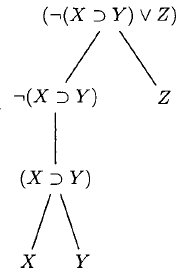
\includegraphics[width=0.3\linewidth]{img/szerkfa}
		\caption{Példa szerkezeti fára.}
		\label{fig:szerkfa}
	\end{figure}
	
	\noindent \textbf{Logikai összetettség}: Egy formula logikai összetettsége a benne található logikai összekötőjelek száma.\\
	
	\noindent \textbf{Művelet hatásköre}: Egy művelet hatásköre a formula részformulái közül az
	a legkisebb logikai összetettségű részformula, melyben az adott művelet előfordul.\\
	
	\noindent \textbf{Fő logikai összekötőjel}: Egy formula fő logikai összekötőjele az az összekötőjel, amelynek
	hatásköre maga a formula.\\
	
	\noindent \textbf{Precedencia}: A logikai összekötőjelek precedenciája csökkenő sorrendben a következő: $\neg, \wedge, \vee, \supset$.\\
	
	A definíciók alapján egyértelmű, hogy egy \textit{teljesen zárójelezett formulában} mi a logikai összekötőjelek hatásköre és mi a fő
	logikai összekötőjel. Most megmutatjuk, hogy egy formulában milyen esetekben és mely részformulákat határoló zárójelek hagyhatóak el úgy, hogy a logikai összekötőjelek hatásköre ne változzon. A részformulák közül a prímformuláknak és a negációs formuláknak nincs külső zárójelpárja, ezért csak az $(A \circ B)$ alakú részformulákról kell eldöntenünk, hogy írható-e helyettük $A \circ B$. A zárójelek elhagyását
	mindig a formula külső zárójelpárjának (ha van ilyen) elhagyásával kezdjük. Majd ha egy részformulában már megvizsgáltuk a külső zárójelelhagyás kérdését, utána ezen részformula közvetlen részformuláinak külső zárójeleivel foglalkozunk. Két eset lehetséges:
	
	\begin{enumerate}
		\item	A részformula egy negációs formula, melyben az $(A \circ B)$ alakú közvetlen részformula külső zárójelei nem hagyhatók el.
		
		\item	A részformula egy $(A \bullet B)$ vagy $A \bullet B$ alakú formula, melynek $A$ és $B$ közvetlen részformuláiban kell dönteni a külső zárójelek sorsáról. Ha az $A$ formula $A_{1} \circ A_{2}$ alakú, akkor $A$ külső zárójelpárja akkor hagyható el, ha $\circ$ nagyobb precedenciájú, mint $\bullet$. Ha a $B$ formula $B_{1} \circ B_{2}$ alakú, akkor $B$ külső zárójelpárja akkor hagyható el, ha $\circ$ nagyobb vagy egyenlő precedenciájú, mint $\bullet$.
		
		\item	Ha egy $(A \wedge B)$ vagy $A \wedge B$ alakú formula valamely közvetlen részformulája szintén konjunkció, illetve egy
		$(A \vee B)$ vagy $A \vee B$ alakú formula valamely közvetlen részformulája szintén diszjunkció, akkor az ilyen részformulákból a külső zárójelpár elhagyható. 
	\end{enumerate}
	
	\noindent \textbf{Formulaláncok}: A zárójelek elhagyására vonatkozó megállapodásokat figyelembe véve úgynevezett konjunkciós, diszjunkciós, illetve implikációs formulaláncokat is nyerhetünk. Ezek alakja $A_{1} \wedge ... \wedge A_{n}$, $A_{1} \vee ... \vee A_{n}$, illetve
	$A_{1} \supset ... \supset A_{n}$ Ezeknek a láncformuláknak a fő logikai összekötőjelét a következő zárójelezési megállapodással fogjuk meghatározni: $(A_{1} \wedge (A_{2} \wedge ... \wedge (A_{n-1} \wedge A_{n})...))$, $(A_{1} \vee (A_{2} \vee ... \vee (A_{n-1} \vee A_{n})...))$, illetve $(A_{1} \supset (A_{2} \supset ... \supset (A_{n-1} \supset A_{n})...))$
	
	\subsubsection{Az ítéletlogika szemantikája}
	
	\noindent \textbf{Interpretáció}: $\mathcal{L}_{0}$ interpretációján egy $\mathcal{I} : V_{v} \to \mathbb{L}$ függvényt értünk, mely minden ítéletváltozóhoz egyértelműen hozzárendel egy igazságértéket.\\
	
	\noindent \textbf{Boole-értékelés}: $\mathcal{L}_{0}$-beli formulák $\mathcal{I}$ \textit{interpretációbeli Boole-értékelése} a következő $\mathcal{B}_{\mathcal{I}} : \mathcal{L}_{0} \to \mathbb{L}$ függvény:
	
	\begin{enumerate}
		\item ha $A$ prímformula, akkor $\mathcal{B}_{\mathcal{I}}(A) = \mathcal{I}(A)$,
		
		\item $\mathcal{B}_{\mathcal{I}}(\neg A)$ legyen $\neg \mathcal{B}_{\mathcal{I}}(A) $,
		
		\item $\mathcal{B}_{\mathcal{I}}(A \wedge B)$ legyen $\mathcal{B}_{\mathcal{I}}(A) \wedge \mathcal{B}_{\mathcal{I}}(B)$,
		
		\item $\mathcal{B}_{\mathcal{I}}(A \vee B)$ legyen $\mathcal{B}_{\mathcal{I}}(A) \vee \mathcal{B}_{\mathcal{I}}(B)$,
		
		\item $\mathcal{B}_{\mathcal{I}}(A \supset B)$ legyen $\mathcal{B}_{\mathcal{I}}(A) \supset \mathcal{B}_{\mathcal{I}}(B)$,
	\end{enumerate}
	
	\noindent \textbf{Bázis}: A formula ítéletváltozóinak egy rögzített sorrendje.\\
	
	\noindent \textbf{Szemantikus fa}: Egy formula különböző interpretációit szemantikus fa segítségével szemléltethetjük. A szemantikus
	fa egy olyan bináris fa, amelynek $i$. szintje ($i>=1$) a bázis $i$. ítéletváltozójához tartozik, és minden csúcsából két él indul, az
	egyik a szinthez rendelt ítéletváltozóval, a másik annak negáltjával címkézve. Az $X$ ítéletváltozó esetén az $X$ címke jelentse azt, hogy az $X$ \textit{igaz} az adott interpretációban, a $\neg X$ címke pedig azt, hogy \textit{hamis} az adott interpretációban. A szemantikus fa
	minden ága egy-egy lehetséges interpretációt reprezentál. Egy $n$ változós formula esetén minden ág $n$ hosszú, és a fának $2^{n}$ ága van és az összes lehetséges interpretációt tartalmazza. 
	
	\begin{figure}[H]
		\centering
		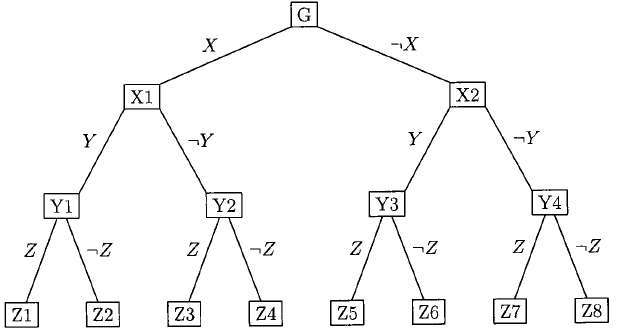
\includegraphics[width=0.6\linewidth]{img/szemantikusfa}
		\caption{Az X,Y,Z ítéletváltozókat tartalmazó formula szemantikus fája.}
		\label{fig:szemantikusfa}
	\end{figure}
	
	\noindent \textbf{Igazságtábla}: Egy $n$ változós formula igazságtáblája egy $n+1$ oszlopból és $2^{n}$ sorból álló táblázat.
	A táblázat fejlécében az $i$. oszlophoz ($1<=i<=n$) a formula bázisának $i$. ítéletváltozója, az $n+1$. oszlophoz maga a formula
	van hozzárendelve. Az első $n$ oszlopban az egyes sorokhoz megadjuk rendre a formula különböző interpretációit, majd a formula
	oszlopába minden sorba beírjuk a formula - a sorhoz tartozó interpretációbeli Boole-értékeléssel kapott - igazságértékét.\\
	
	\noindent \textbf{A logikai műveletek igazságtáblája}:
	
	\begin{table}[H]
		\begin{tabular}{ll|lllll}
			X & Y & $\neg X$ & $X \wedge Y$ & $X \vee Y$  & $ X \supset Y$ &  \\ \hline
			i & i & h & i & i & i &  \\
			i & h & h & h & i & h &  \\
			h & i & i & h & i & i &  \\
			h & h & i & h & h & i & 
		\end{tabular}
	\end{table}
	
	\noindent \textbf{Igazhalmaz, hamishalmaz}: Egy $A$ formula igazhalmaza $(A^{i})$
	azon interpretációk halmaza, melyen a formula igazságértékelése igaz. Az $A$ formula
	hamishalmaza $(A^{h})$ pedig azon interpretációk halmaza, melyekre a formula igazságértékelése hamis.\\
	
	\noindent \textbf{Igazságértékelés függvény}:  Olyan függvény, amely minden formulához hozzárendeli az igazhalmazát ($\varphi A^{i}$) vagy
	a hamishalmazát ($\varphi A^{h}$).\\
	
	Legyen $A$ egy tetszőleges ítéletlogikai formula. Határozzuk meg $A$-hoz az interpretációira vonatkozó $\varphi A^{i}$, illetve
	$\varphi A^{h}$ feltételeket a következőképpen:
	
	\begin{enumerate}
		\item	Ha $A$ prímformula, a $\varphi A^{i}$ feltételt pontosan azok az $\mathcal{I}$ interpretációk elégítik ki,  melyekre
		$\mathcal{I}(A)=igaz$, a $\varphi A^{h}$ feltételt pedig pontosan azok melyekre	$\mathcal{I}(A)=hamis$.
		
		\item	A $\varphi (\neg A)^{i}$ feltételek pontosan akkor teljesülnek, ha teljesülnek a $\varphi A^{h}$ feltételek.
		
		\item	A $\varphi (A \wedge B)^{i}$ feltételek pontosan akkor teljesülnek, ha a $\varphi A^{i}$ és a $\varphi B^{i}$ feltételek egyszerre teljesülnek.
		
		\item	A $\varphi (A \vee B)^{i}$ feltételek pontosan akkor teljesülnek, ha a $\varphi A^{i}$ vagy a $\varphi B^{i}$ feltételek teljesülnek.
		
		\item	A $\varphi (A \supset B)^{i}$ feltételek pontosan akkor teljesülnek, ha a $\varphi A^{h}$ vagy a $\varphi B^{i}$ feltételek teljesülnek.
	\end{enumerate}	
	
	\noindent \textbf{Tétel}: Tetszőleges $A$ ítéletlogikai formula esetén a  $\varphi A^{i}$ feltételeket pontosan az  $A^{i}$-beli
	interpretációk teljesítik.\\
	
	\noindent \textbf{Igazságértékelés-fa}:  Egy $A$ formula $\varphi A^{i}$, illetve $\varphi A^{h}$ feltételeket kielégítő interpretációit
	az igazságértékelés-fa segítségével szemléltethetjük. Az igazságértékelés-fát a formula szerkezeti fájának felhasználásával állítjuk elő.
	A gyökérhez hozzárendeljük, hogy $A$ melyik igazságértékre való igazságértékelés-feltételeit keressük, majd a gyökér alá $A$ közvetlen részformulái kerülnek a megfelelő feltétel-előírással, az alábbiak szerint:
	
	\begin{figure}[H]
		\centering
		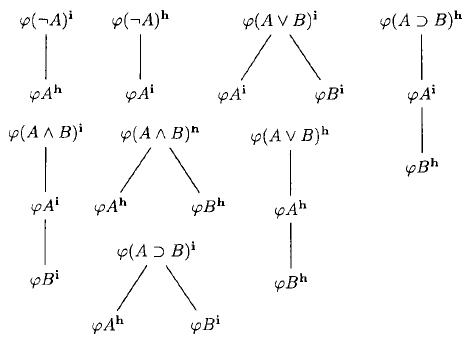
\includegraphics[width=0.7\linewidth]{img/igazsagertfa}
		\caption{Igazságértékelés-fa feltétel-előírásai.}
		\label{fig:igazsagertfa}
	\end{figure}
	
	Ezután a gyökérhez a \checkmark (feldolgozott) jelet rendeljük. Az eljárást rekurzívan folytatjuk, amíg egy ágon a fel nem dolgozott
	formulák
	
	\begin{itemize}
		\item	(a) mind ítéletváltozók nem lesznek, vagy
		
		\item	(b) ugyanarra a formulára egymásnak ellentmondó előírás nem jelenik meg. 
	\end{itemize}
	
	Az (a) esetben az ágon előforduló ítéletváltozóknak az ágon rögzített igazságértékeit tartalmazó $n$-esek mind elemei $\varphi A^{i}$
	gyökér esetén a formula igazhalmazának, $\varphi A^{h}$ gyökér esetén a formula hamishalmazának.
	
	A (b) esetben nem áll elő ilyen igazságérték $n$-es.
	
	\begin{figure}[H]
		\centering
		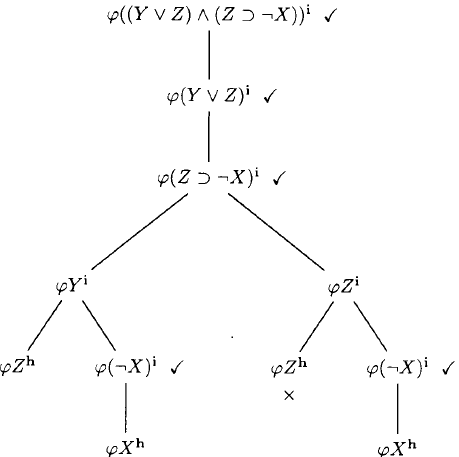
\includegraphics[width=0.5\linewidth]{img/igazsagertfapelda}
		\caption{Az $(Y \vee Z) \wedge (Z \supset \neg X)$ formula igazságértékelés-fája.}
		\label{fig:igazsagertfapelda}
	\end{figure}
	
	\noindent A fenti példában a formula igazhalmaza az igazságértékelés-fa alapján: $\left\{(i,i,h),(h,i,i),(h,i,h),(h,h,i)\right\}$\\

	\noindent \textbf{Kiterjesztett igazságtábla}: Egy igazságtáblában a formula igazságértéke kiszámításának megkönnyítésére vezették
	be a kiterjesztett igazságtáblát. A kiterjesztett igazságtáblában az ítéletváltozókhoz és a formulához rendelt oszlopokon kívül rendre
	a formula részformuláihoz tartozó oszlopok is megjelennek. Tulajdonképpen a szerkezeti fában megjelenő részformulák vannak felsorolva.
	
	\begin{figure}[H]
		\centering
		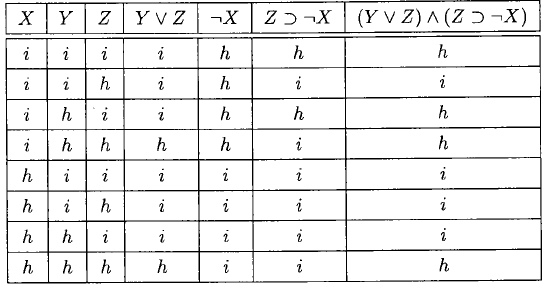
\includegraphics[width=0.5\linewidth]{img/kiterjigaztabla}
		\caption{Az $(Y \vee Z) \wedge (Z \supset \neg X)$ formula kiterjesztett igazságtáblája.}
		\label{fig:kiterjigaztabla}
	\end{figure}
	
	\noindent \textbf{Formula kielégíthetősége, modellje}: Egy $A$ ítéletlogikai formula \textit{kielégíthető}, ha létezik olyan  $\mathcal{I}$
	interpretáció, melyre $\mathcal{I} \models_{0} A$, azaz a $\mathcal{B}_{\mathcal{I}}$ Boole-értékelés $A$-hoz igaz értéket rendel. Egy
	ilyen interpretációt $A$ \textit{modelljének} nevezünk. Ha $A$-nak nincs modellje, akkor azt mondjuk, hogy \textit{kielégíthetetlen}.
	
	Ha $A$ igazságtáblájában van olyan sor, amelyben a formula oszlopában igaz érték szerepel, akkor a formula kielégíthető, különben kielégíthetetlen. Ugyanígy, ha $\varphi A^{i}$ nem üres, akkor kielégíthető, különben kielégíthetetlen.\\
	
	\noindent \textbf{Ítéletlogikai törvény, tautológia}: Egy $A$ ítéletlogikai formula \textit{ítéletlogikai törvény} vagy másképpen \textit{tautológia}, ha $\mathcal{L}_{0}$ minden interpretációja modellje $A$-nak. (jelölés: $\models_{0} A$)\\
	
	\noindent \textbf{Eldöntésprobléma}: Eldöntésproblémának nevezzük a következő feladatokat:
	\begin{enumerate}
		\item	Döntsük el tetszőleges formuláról, hogy tautológia-e!
		
		\item	Döntsük el tetszőleges formuláról, hogy kielégíthetetlen-e!
	\end{enumerate}
	
	\noindent \textbf{Tautologikusan ekvivalens formulák}: Az $A$ és $B$ ítéletlogikai formulák \textit{tautologikusan ekvivalensek} (jelölés: $A \sim _{0} B$), ha $\mathcal{L}_{0}$ minden $\mathcal{I}$ interpretációjában $\mathcal{B}_{\mathcal{I}}(A)=\mathcal{B}_{\mathcal{I}}(B)$.\\
	
	\noindent \textbf{Formulahalmaz kielégíthetősége, modellje}: $\mathcal{L}_{0}$ formuláinak egy tetszőleges $\Gamma$ halmaza
	kielégíthető, ha van $\mathcal{L}_{0}$-nak olyan $\mathcal{I}$ interpretációja, melyre: $\forall A \in \Gamma: \mathcal{I} \models_{0} A$.
	Egy ilyen $\mathcal{I}$ interpretáció modellje $\Gamma$-nak. Ha $\Gamma$-nak nincs modellje, akkor $\Gamma$ kielégíthetetlen.\\
	
	\noindent \textbf{Lemma}: Egy $\left\{A_{1},A_{2},...,A_{n}\right\}$ formulahalmaznak pontosan azok az $\mathcal{I}$ interpretációk
	a modelljei, amelyek a $A_{1} \wedge A_{2} \wedge ... \wedge A_{n}$ formulának. Következésképpen $\left\{A_{1},A_{2},...,A_{n}\right\}$
	pontosan akkor kielégíthetetlen, ha az $A_{1} \wedge A_{2} \wedge ... \wedge A_{n}$ formula kielégíthetlen.\\
	
	\noindent \textbf{Szemantikus következmény}: Legyen $\Gamma$ ítéletlogikai formulák tetszőleges halmaza, $B$ egy tetszőleges formula.
	Azt mondjuk, hogy a $B$ formula \textit{tautologikus következménye} a $\Gamma$ formulahalmaznak (jelölés: $\Gamma \models_{0} B$), ha minden olyan interpretáció, amely modellje $\Gamma$-nak, modellje $B$-nek is. A $\Gamma$-beli formulákat feltételformuláknak, vagy premisszáknak,
	a B formulát következményformulának (konklúziónak) hívjuk.\\
	
	\noindent \textbf{Tétel}: Legyen $\Gamma$ ítéletlogikai formulák tetszőleges halmaza, $A$,$B$,$C$ tetszőleges ítéletlogikai formulák.
	Ha $\Gamma \models_{0} A$, $\Gamma \models_{0} B$ és $\left\{A,B\right\} \models_{0} C$, akkor $\Gamma \models_{0} C$.\\
	
	\noindent \textbf{Tétel}: Legyenek $A_{1},A_{2},...,A_{n}, B$ tetszőleges ítéletlogikai formulák.
	$\left\{A_{1},A_{2},...,A_{n}\right\} \models_{0} B$ pontosan akkor, ha a $\left\{A_{1},A_{2},...,A_{n}, \neg B\right\}$
	formulahalmaz kielégíthetetlen, azaz a $A_{1} \wedge A_{2} \wedge ... \wedge A_{n} \wedge \neg B$ formula kielégíthetetlen.\\
	
	\noindent \textbf{Tétel}: Legyenek $A_{1},A_{2},...,A_{n}, B$ tetszőleges ítéletlogikai formulák.
	$\left\{A_{1},A_{2},...,A_{n}\right\} \models_{0} B$ pontosan akkor, ha
	$\models_{0} A_{1} \wedge A_{2} \wedge ... \wedge A_{n} \supset B$.\\
	
	\paragraph{Ekvivalens átalakítások}
	Fogalmak:
	\begin{enumerate}
		\item	Egy prímformulát (ítéletváltozót), vagy annak a negáltját közös néven \textit{literálnak} nevezünk. A prímformula
		a \textit{literál alapja}. Egy literált bizonyos esetekben \textit{egységkonjunkciónak} vagy \textit{egységdiszjunkciónak}
		(\textit{egységklóznak}) is hívunk.
		
		\item	\textit{Elemi konjunkció} az egységkonjunkció, illetve a különböző alapú literálok konjunkciója ($\wedge$ kapcsolat
		a literálok között). \textit{Elemi diszjunkció} vagy \textit{klóz} az egységdiszjunkció és a különböző alapú literálok
		diszjunkciója ($\vee$ kapcsolat a literálok között). Egy elemi konjunkció, illetve elemi diszjunkció \textit{teljes}
		egy $n$-változós logikai műveletre nézve, ha mind az $n$ ítéletváltozó alapja valamely literáljának.
		
		\item	\textit{Diszjunktív normálformának} (DNF) nevezzük az elemi konjunkciók diszjunkcióját. 
		\textit{Konjunktív normálformának} (KNF) nevezzük az elemi diszjunkciók konjunkcióját. \textit{Kitüntetett}
		diszjunktív, illetve konjunktív normálformákról (KDNF, ileltve KKNF) beszélünk, ha a bennük szereplő
		elemi konjunkciók, illetve elemi diszjunkciók teljesek.
	
	\end{enumerate}	
	
	\noindent \textbf{Tetszőleges logikai műveletet leíró KDNF, KKNF előállítása}:	Legyen $b: \mathbb{L}^{n} \to \mathbb{L}$
	egy $n$-változós logikai művelet. Adjuk meg $b$ művelettábláját.
	Az első $n$ oszlop fejlécébe az $X_{1}$, $X_{2}$, ... $X_{n}$ ítéletváltozókat írjuk.\\
	
	\noindent A $b$-t leíró KDNF előállítása:
	
	\begin{enumerate}
		\item	Válasszuk ki azokat a sorokat a művelettáblában, ahol az adott igazságérték $n$-eshez $b$ \textit{igaz}
		értéket rendel hozzá. Legyenek ezek a sorok rendre $s_{1}, s_{2}, .. s_{r}$. Minden ilyen sorhoz rendeljünk
		hozzá egy $X_{1}' \wedge X_{2}' \wedge ... \wedge X_{n}'$ teljes elemi konjunkciót úgy, hogy az $X_{j}'$ literál
		$X_{j}$ vagy $\neg X_{j}$ legyen aszerint, hogy ebben a sorban $X_{j}$ \textit{igaz} vagy \textit{hamis} igazságérték
		szerepel. Az így nyert teljes elemi konjunkciók legyenek rendre $k_{s_{1}}, k_{s_{2}}, .. k_{s_{r}}$.
		
		\item	Az így kapott teljes elemi konjunkciókból készítsünk egy diszjunkciós láncformulát:
		$k_{s_{1}} \vee k_{s_{2}} \vee ... \vee k_{s_{r}}$. Ez a formula lesz a $b$ művelet kitüntetett diszjunktív
		normálformája (KDNF).
	\end{enumerate}
	
	\begin{figure}[H]
		\centering
		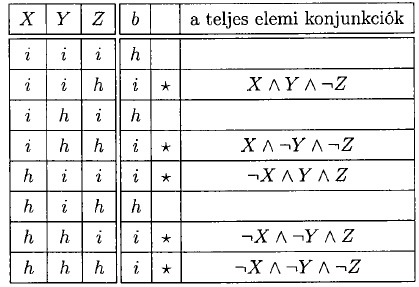
\includegraphics[width=0.5\linewidth]{img/kdnf_pelda}
		\caption{Egy háromváltozós $b$ logikai művelet művelettáblája és az előállított teljes elemi konjunkciók.}
		\label{fig:kdnf_pelda}
	\end{figure}
	
	A fenti példa $b$ műveletének kitüntetett diszjunktív normálformája a következő formula:\\
	$(X \wedge Y \wedge \neg Z) \vee (X \wedge \neg Y \wedge \neg Z) \vee (\neg X \wedge Y \wedge Z) \vee (\neg X \wedge \neg Y \wedge Z) \vee (\neg X \wedge \neg Y \wedge \neg Z)$.\\
	
	\noindent A $b$-t leíró KKNF előállítása:
	
	\begin{enumerate}
		\item	Válasszuk ki azokat a sorokat a művelettáblában, ahol az adott igazságérték $n$-eshez $b$ \textit{hamis}
		értéket rendel hozzá. Legyenek ezek a sorok rendre $s_{1}, s_{2}, .. s_{r}$. Minden ilyen sorhoz rendeljünk
		hozzá egy $X_{1}' \vee X_{2}' \vee ... \vee X_{n}'$ teljes elemi diszjunkciót úgy, hogy az $X_{j}'$ literál
		$X_{j}$ vagy $\neg X_{j}$ legyen aszerint, hogy ebben a sorban $X_{j}$ \textit{hamis} vagy \textit{igaz} igazságérték
		szerepel. Az így nyert teljes elemi diszjunkciók legyenek rendre $d_{s_{1}}, d_{s_{2}}, .. d_{s_{r}}$.
		
		\item	Az így kapott teljes elemi diszjunkciókból készítsünk egy konjunkciós láncformulát:
		$d_{s_{1}} \wedge d_{s_{2}} \wedge ... \wedge d_{s_{r}}$. Ez a formula lesz a $b$ művelet kitüntetett konjunktív
		normálformája (KKNF).
	\end{enumerate}
	
	\begin{figure}[H]
		\centering
		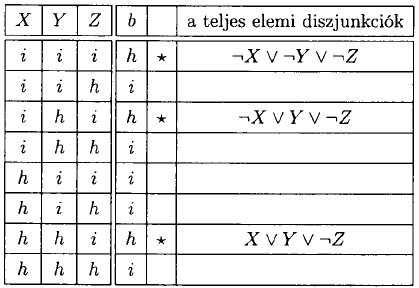
\includegraphics[width=0.5\linewidth]{img/kknf_pelda}
		\caption{Egy háromváltozós $b$ logikai művelet művelettáblája és az előállított teljes elemi diszjunkciók.}
		\label{fig:kknf_pelda}
	\end{figure}
	
	A fenti példa $b$ műveletének kitüntetett konjunktív normálformája a következő formula:\\
	$(\neg X \vee \neg Y \vee \neg Z) \wedge (\neg X \vee Y \vee \neg Z) \wedge (X \vee Y \vee \neg Z)$. \\
	
	\noindent \textbf{KNF, DNF egyszerűsítése}: Egy ítéletlogikai formula logikai összetettségén a formulában szereplő
	logikai összekötőjelek számát értettük. Ugyanazt a logikai műveletet leíró formulák közül azt tekintjük egyszerűbbnek,
	amelynek kisebb a logikai összetettsége (azaz kevesebb logikai összekötőjelet tartalmaz).
	
	Legyen $X$ egy ítéletváltozó $k$ egy az $X$-et nem tartalmazó elemi konjunkció, $d$ egy $X$-et nem tartalmazó elemi
	diszjunkció. Ekkor az
	
	\begin{itemize}
		\item	(a) $(X \wedge k) \vee (\neg X \wedge k) \sim_{0} k $ és
		
		\item	(b) $(X \vee d) \wedge (\neg X \vee d) \sim_{0} d $
	\end{itemize}
	
	egyszerűsítési szabályok alkalmazásával konjunktív és diszjunktív normálformákat írhatunk át egyszerűbb alakba.\\
	
	\noindent Klasszikus Quine--McCluskey-féle algoritmus KDNF egyszerűsítésére:
	
	\begin{enumerate}
		\item	Soroljuk fel a KDNF-ben szereplő összes teljes elemi konjunkciót az $L_{0}$ listában, $j:=0$.
		
		\item	Megvizsgáljuk az $L_{j}$-ben szereplő összes lehetséges elemi konjunkciópárt, hogy alkalmazható-e
		rájuk az (a) egyszerűsítési szabály. Ha igen, akkor a két kiválasztott konjunkciót $\checkmark$-val megjelöljük,
		és az eredmény konjunkciót beírjuk a $L_{j+1}$ listába. Azok az elemi konjunkciók, amelyek az $L_{j}$ vizsgálata
		során nem lesznek megjelölve, nem voltak egyszerűsíthetők, tehát bekerülnek az egyszerűsített diszjunktív
		normálformába.
		
		\item	Ha az $L_{j+1}$ konjunkciólista nem üres, akkor $j:=j+1$. Hajtsuk végre újból a 2. lépést.
		
		\item	Az algoritmus során kapott, de meg nem jelölt elemi konjunkciókból készítsünk egy diszjunkciós
		láncformulát. Így az eredeti KDNF-el logikailag ekvivalens, egyszerűsített DNF-et kapunk.
	\end{enumerate}
	
	\paragraph{Rezolúció}
	
	Legyenek $A_{1}, A_{2}, ... , A_{n}, B$ tetszőleges ítéletlogikai formulák.
	Azt szeretnénk bebizonyítani, hogy $\left\{A_{1}, A_{2}, ... , A_{n}\right\} \models_{0} B$,
	ami ekvivalens azzal, hogy $\left\{A_{1}, A_{2}, ... , A_{n}, \neg B\right\}$ kielégíthetetlen.
	Írjuk át ez utóbbi formulahalmaz formuláit KNF alakba! Ekkor a
	$\left\{KNF_{A_{1}}, KNF_{A_{2}}, ... , KNF_{A_{n}}, KNF_{\neg B}\right\}$ formulahalmazt
	kapjuk, ami pontosan akkor kielégíthetetlen, ha a halmaz formuláiban szereplő klózok halmaza
	kielégíthetetlen.
	
	A klózokra vonatkozó egyszerűsítési szabály szerint ha $X$ ítéletváltozó, $C$ pedig $X$-et nem
	tartalmazó klóz, akkor $(X \vee C) \wedge (\neg X \vee C) \sim_{0} C$. Az $X$ és a $\neg X$
	egységklózok (azt mondjuk, hogy $X$ és $\neg X$ komplemens literálpár) konjunkciójával ekvivalens
	egyszerűbb, egyetlen literált sem tartalmazó klóz az üres klóz, melyet a $\square$ jellel
	jelölünk és definíció szerint minden interpretációban hamis igazságértékű.
	
	Legyenek most $C_{1}$ és $C_{2}$ olyan klózok, melyek pontosan egy komplemens literálpárt tartalmaznak,
	azaz $C_{1} = C_{1}' \vee L_{1}$ és $C_{2} = C_{2}' \vee L_{2}$, ahol $L_{1}$ és $L_{2}$ az egyetlen
	komplemens literálpár ($C_{1}'$ és $C_{2}'$ üres klózok is lehetnek). Világos, hogy ha a két klózban
	a komplemens literálpáron kívül is vannak literálok, és ezek nem mind azonosak, az egyszerűsítési
	szabály alkalmazhatósági feltétele nem áll fenn.\\
	
	\noindent \textbf{Tétel}: Ha $C_{1} = C_{1}' \vee L_{1}$ és $C_{2} = C_{2}' \vee L_{2}$,
	ahol $L_{1}$ és $L_{2}$	komplemens literálpár, akkor $\left\{C_{1},C_{2}\right\} \models_{0} C_{1}' \vee C_{2}'$\\
	
	\noindent \textbf{Rezolvens}: Legyenek $C_{1}$ és $C_{2}$ olyan klózok, melyek pontosan egy komplemens literálpárt tartalmaznak,
	azaz $C_{1} = C_{1}' \vee L_{1}$ és $C_{2} = C_{2}' \vee L_{2}$, ahol $L_{1}$ és $L_{2}$ a komplemens literálpár,
	a $C_{1}' \vee C_{2}'$ klózt a $(C_{1},C_{2})$ klózpár (vagy a $C_{1} \vee C_{2}$ formula) \textit{rezolvensének} nevezzük.
	Ha $C_{1} = L_{1}$ és $C_{2} = L_{2}$ (azaz $C_{1}'$ és $C_{2}'$ üres klózok), rezolvensük az üres klóz ($\square$).
	Az a tevékenység, melynek eredménye a rezolvens, a \textit{rezolválás}.
	
	\begin{figure}[H]
		\centering
		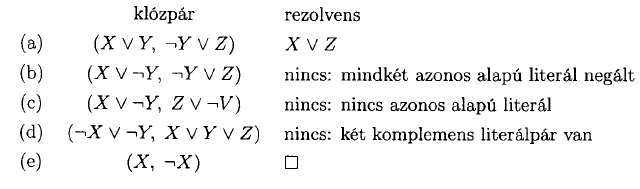
\includegraphics[width=0.7\linewidth]{img/rezolvens}
		\caption{Példák klózpárok rezolválhatóságára, rezolvensére.}
		\label{fig:rezolvens}
	\end{figure}
	
	\noindent \textbf{Tétel}: Ha a $C$ klóz a $(C_{1},C_{2})$ klózpár rezolvense, akkor azon $\mathcal{I}$ interpretációk
	a $\left\{C_{1}, C_{2}\right\}$ klózhalmazt nem elégíthetik ki, amelyekben $C$ igazságértéke hamis, azaz
	$\mathcal{B}_{\mathcal{I}}(C) = hamis$.\\
	
	\noindent \textbf{Rezolúciós levezetés}: Egy $S$ klózhalmazból a $C$ klóz rezolúciós levezetése egy olyan véges
	$k_{1}, k_{2}, ... ,k_{m} (m \geq 1)$ klózsorozat, ahol minden $j = 1, 2, ..., m$-re
	
	\begin{enumerate}
		\item	vagy $k_{j} \in S$,
		
		\item	vagy van olyan $1 \leq s,t \le j$, hogy $k_{j}$ a $(k_{s}, k_{t})$ klózpár rezolvense,
	\end{enumerate}
	
	\noindent és a klózsorozat utolsó tagja, $k_{m}$, éppen a $C$ klóz.
	 
	Megállapodásunk szerint a rezolúciós kalkulus eldöntésproblémája az, hogy levezethető-e $S$-ből $\square$. A
	rezolúciós levezetés célja tehát $\square$ levezetése $S$-ből. Azt, hogy $\square$ levezethető $S$-ből,
	úgy is ki lehet fejezni, hogy létezik $S$-nek rezolúciós cáfolata.\\
	
	\noindent Példa: Próbáljuk meg levezetni $\square$-t az
	$S = \left\{\neg X \vee Y, \neg Y \vee Z, X \vee Z, \neg V \vee Y \vee Z, \neg Z \right\}$
	klózhalmazból. A levezetés bármelyik $S$-beli klózból indítható.
	
	\begin{figure}[H]
		\centering
		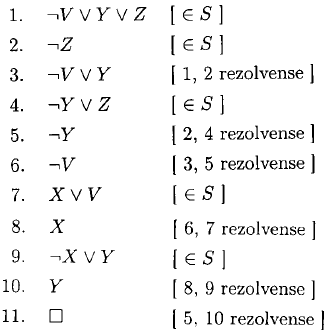
\includegraphics[width=0.4\linewidth]{img/rezoluciopelda}
		\caption{$\square$ rezolúciós levezetése $S$-ből.}
		\label{fig:rezoluciopelda}
	\end{figure}
	 
	\noindent \textbf{Lemma}: Legyen $S$ tetszőleges klózhalmaz. $S$-ből történő rezolúciós levezetés esetén bármely $S$-ből
	levezetett klóz tautologikus következménye $S$-nek.\\
	
	\noindent \textbf{A rezolúciós kalkulus helyessége}: A rezolúciós kalkulus \textit{helyes}, azaz tetszőleges
	$S$ klózhalmaz esetén amennyiben $S$-ből levezethető $\square$, akkor $S$ \textit{kielégíthetetlen}.\\
	 
	\noindent \textbf{A rezolúciós kalkulus teljessége}: A rezolúciós kalkulus \textit{teljes}, azaz bármely véges, kielégíthetetlen
	$S$ klózhalmaz esetén $S$-ből levezethető $\square$.\\	 
	 
	\noindent \textbf{Levezetési fa}: Egy rezolúciós levezetés szerkezetét \textit{levezetési fa} segítségével szemléltethetjük.
	A levezetési fa csúcsai klózok. Két csúcsból pontosan akkor vezet él egy harmadik, közös csúcsba, ha az a két klóz rezolvense.
	
	\begin{figure}[H]
		\centering
		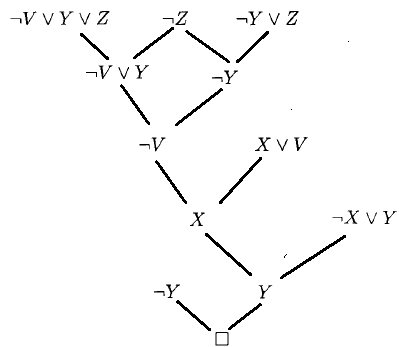
\includegraphics[width=0.5\linewidth]{img/rezoluciopelda_levfa}
		\caption{Az előző példa levezetési fája.}
		\label{fig:rezoluciopelda_levfa}
	\end{figure}
	
	\noindent \textbf{Rezolúciós stratégiák}:
	
	\begin{itemize}
		\item	\textit{Lineáris rezolúció}: Egy $S$ klózhalmazból való lineáris rezolúciós levezetés egy olyan
		$k_{1},l_{1},k_{2},l_{2}, ..., k_{m-1},l_{m-1}, k_{m}$ rezolúciós levezetés, amelyben minden
		$j = 2, 3, ..., m$-re $k_{j}$ a $(k_{j-1},l_{j-1})$ klózpár rezolvense. A $k_{j}$ klózokat centrális
		klózoknak, az $l_{j}$ klózokat mellékklózoknak nevezzük.		
		
		Tetszőleges rezolúciós levezetés átírható lineárissá, azaz a lineáris rezolúciós kalkulus teljes.
		
		\item	\textit{Lineáris inputrezolúció}: Egy $S$ klózhalmazból való lineáris inputrezolúciós levezetés
		egy olyan $k_{1},l_{1},k_{2},l_{2}, ..., k_{m-1},l_{m-1}, k_{m}$ lineáris rezolúciós levezetés, amelyben minden
		$j = 1, 2, ..., m-1$-re $l_{j} \in S$, azaz a lineáris inputrezolúciós levezetésben a mellékklózok $S$ elemei.
		
		A lineáris inputrezolúciós stratégia nem teljes, de megadható olyan formulaosztály, melyre az. A legfeljebb egy
		negált literált tartalmazó klózokat Horn-klózoknak nevezzük, a Horn-formulák pedig azok a formulák, melyek
		konjunktív normálformája Horn-klózok konjunkciója. A lineáris inputrezolúciós stratégia Horn-formulák esetén teljes.
	\end{itemize}
	
	\subsection{Predikátumkalkulus}
	
	\subsubsection{Elsőrendű logikai nyelvek szintaxisa}
	
	Egy elsőrendű logikai nyelv ábécéje logikai és logikán kívüli szimbólumokat, továbbá elválasztójeleket tartalmaz.
	A logikán kívüli szimbólumhalmaz megadható $<Srt, Pr, Fn, Cnst>$ alakban, ahol:
	
	\begin{enumerate}
		\item	$Srt$ nemüres halmaz, elemei fajtákat szimbolizálnak,
		
		\item	$Pr$ nemüres halmaz, elemei predikátumszimbólumok,
		
		\item	az $Fn$ halmaz elemei függvényszimbólumok,
		
		\item	$Cnst$ pedig a függvényszimbólumok halmaza.
	\end{enumerate}
	
	\noindent Az $<Srt, Pr, Fn, Cnst>$ ábécé szignatúrája egy $<\nu_{1}, \nu_{2}, \nu_{3}>$ hármas, ahol
	
	\begin{enumerate}
		\item	minden $P \in Pr$ predikátumszimbólumhoz $\nu_{1}$ a predikátumszimbólum alakját,
		azaz a $(\pi_{1}, \pi_{2}, ..., \pi_{k})$ fajtasorozatot,
		
		\item	minden $f \in Fn$ függvényszimbólumhoz $\nu_{2}$ a függvényszimbólum alakját,
		azaz a $(\pi_{1}, \pi_{2}, ..., \pi_{k}, \pi)$ fajtasorozatot és

		\item	minden $c \in Cnst$ konstansszimbólumhoz $\nu_{3}$ a konstansszimbólumhoz alakját,
		azaz $(\pi)$-t
	\end{enumerate}
	
	\noindent rendel ($k > 0$ és $\pi_{1}, \pi_{2}, ..., \pi_{k}, \pi \in Srt$). 
	
	Logikai jelek az ítéletlogikában is használt logikai összekötőjelek, valamint az univerzális ($\forall$)
	és egzisztenciális ($\exists$) kvantorok és a különböző fajtájú individuumváltozók. Egy elsőrendű
	nyelv ábécéjében minden $\pi \in Srt$ fajtához szimbólumoknak megszámlálhatóan végtelen
	$v_{1}^{\pi}, v_{2}^{\pi}, ...$ rendszere tartozik, ezeket a szimbólumokat nevezzük $\pi$ fajtájú
	változóknak. Elválasztójel a nyitó és csukó zárójelek, és a vessző.
	
	Az elsőrendű logikai nyelvekben az elválasztójelek és a logikai jelek mindig ugyanazok, viszont
	a logikán kívüli jelek halmaza, illetve ezek szignatúrája nyelvről nyelvre lényegesen különbözhet.
	Ezért mindig megadjuk a $<Srt, Pr, Fn, Cnst>$ négyest és ennek $<\nu_{1}, \nu_{2}, \nu_{3}>$
	szignatúráját, amikor egy elsőrendű logikai nyelv ábécéjére hivatkozunk. Jelölése $V[V_{\nu}]$,
	ahol $V_{\nu}$ adja meg a $<\nu_{1}, \nu_{2}, \nu_{3}>$ szignatúrájú $<Srt, Pr, Fn, Cnst>$ négyest.\\
	
	\noindent \textbf{Termek}: A $V[V_{\nu}]$ ábécé feletti termek halmaza $\mathcal{L}_{t}[V_{\nu}]$, ami
	a következő tulajdonságokkal bír:
	
	\begin{enumerate}
		\item	Minden $\pi \in Srt$ fajtájú változó és konstans $\pi$ fajtájú term.
		
		\item	Ha az $f \in Fn$ függvényszimbólum $(\pi_{1}, \pi_{2}, ..., \pi_{k}, \pi)$ alakú
		és $t_{1}, t_{2}, ..., t_{k}$ -- rendre $\pi_{1}, \pi_{2}, ..., \pi_{k}$ fajtájú -- termek,
		akkor az $f(s_{1}, s_{2}, ..., s_{k})$ egy $\pi$ fajtájú term.
		
		\item	Minden term az 1-2. szabályok véges sokszori alkalmazásával áll elő.
	\end{enumerate}
	
	\noindent \textbf{Formulák}: A $V[V_{\nu}]$ ábécé feletti elsőrendű formulák halmaza $\mathcal{L}_{f}[V_{\nu}]$, ami
	a következő tulajdonságokkal bír:
	
	\begin{enumerate}
		\item	Ha a $P \in Pr$ predikátumszimbólum $(\pi_{1}, \pi_{2}, ..., \pi_{k})$ alakú
		és az $t_{1}, t_{2}, ..., t_{k}$ -- rendre $\pi_{1}, \pi_{2}, ..., \pi_{k}$ fajtájú --
		termek, akkor a $P(t_{1}, t_{2}, ..., t_{k})$ szó egy elsőrendű formula.
		Az így nyert formulákat atomi formuláknak nevezzük.
		
		\item	Ha $S$ elsőrendű formula, akkor $\neg S$ is az.
		
		\item	Ha $S$ és $T$ elsőrendű formulák és $\circ$ binér logikai összekötőjel,
		akkor $(S \circ T)$ is elsőrendű formula.
		
		\item	Ha $S$ eleme elsőrendű formula, $Q$ kvantor ($\forall$ vagy $\exists$) és $x$
		tetszőleges változó, akkor $QxS$ is elsőrendű formula. Az így nyert formulákat kvantált formuláknak nevezzük,
		a $\forall xS$ alakú formulák univerzálisan kvantált formulák, a $\exists xS$ alakú formulák
		pedig egzisztenciálisan kvantált formulák. A kvantált formulákban $Qx$ a formula prefixe, $S$
		pedig a magja.
		
		\item	Minden elsőrendű formula az 1-4. szabályok véges sokszori alkalmazásával áll elő.
	\end{enumerate}
	
	\noindent A $V[V_{\nu}]$ ábécé feletti elsőrendű logikai nyelv
	$\mathcal{L}[V_{\nu}] = \mathcal{L}_{t}[V_{\nu}] \cup \mathcal{L}_{f}[V_{\nu}]$, azaz $\mathcal{L}[V_{\nu}]$
	minden szava vagy term, vagy formula.\\
	
	A negációs, konjunkciós, diszjunkciós, implikációs (ezek jelentése ua., mint nulladrendben) és kvantált formulák
	összetett formulák.
	
	Az elsőrendű logikai nyelv prímformulái az atomi formulák és a kvantált formulák.\\
	
	\noindent \textbf{Változóelőfordulás fajtái}: Egy formula $x$ változójának egy előfordulása:
	
	\begin{itemize}
		\item	szabad, ha nem esik $x$-re vonatkozó kvantor hatáskörébe,
		
		\item	kötött, ha $x$-re vonatkozó kvantor hatáskörébe esik. 
	\end{itemize}
	
	\noindent \textbf{Változó fajtái}: Egy formula $x$ változója:
	
	\begin{itemize}
		\item	szabad, ha minden előfordulása szabad,
		
		\item	kötött, ha minden előfordulása kötött, és
		
		\item	vegyes, ha van szabad és kötött előfordulása is. 
	\end{itemize}
	
	\noindent \textbf{Formula zártsága, nyíltsága}: Egy formula:
	
	\begin{itemize}
		\item	zárt, ha minden változója kötött,
		
		\item	nyílt, ha legalább egy változójának van szabad előfordulása és
		
		\item	kvantormentes, ha nincs benne kvantor
	\end{itemize}
	
	Megjegyzés: a zárt formulák elsőrendű állításokat szimbolizálnak (egy elsőrendű állítás nem más, mint elemek egy halmazára
	megfogalmazott kijelentő mondat).
	
	\subsubsection{Az elsőrendű logika szemantikája}
	
	\noindent \textbf{Matematikai struktúra}: Matematikai struktúrán egy $<U, R, M, K>$ négyest értünk, ahol:
	
	\begin{enumerate}
		\item	$U = \bigcup_{\pi} U_{\pi}$ nem üres alaphalmaz (univerzum),
		
		\item	$R$ az $U$-n értelmezett logikai függvények (relációk) halmaza,
		
		\item	$M$ az $U$-n értelmezett matematikai függvények (alapműveletek) halmaza,
		
		\item	$K$ az $U$ kijelölt elemeinek (konstansainak) halmaza (lehet üres).
	\end{enumerate}
	
	\noindent \textbf{Interpretáció}: Az interpretáció egy $<U, R, M, K>$ matematikai struktúra és
	$\mathcal{I} = <\mathcal{I}_{Srt}, \mathcal{I}_{Pr}, \mathcal{I}_{Fn}, \mathcal{I}_{Cnst}>$
	függvénynégyes, ahol:
	
	\begin{itemize}
		\item	az $\mathcal{I}_{Srt} : \pi \mapsto U_{\pi}$ függvény megad minden egyes $\pi \in Srt$ fajtához
		egy $U_{\pi}$ nemüres halmazt, a $\pi$ fajtájú individuumok halmazát,
		
		\item	az $\mathcal{I}_{Pr} : P \mapsto P^{\mathcal{I}}$ függvény megad minden
		$(\pi_{1}, \pi_{2}, ..., \pi_{k})$ alakú $P \in Pr$ predikátumszimbólumhoz egy
		$P^{\mathcal{I}} : U_{\pi_{1}} \times U_{\pi_{2}} \times ... \times U_{\pi_{k}} \to \mathbb{L}$
		logikai függvényt (relációt),
		
		\item	az $\mathcal{I}_{Fn} : f \mapsto f^{\mathcal{I}}$ függvény hozzárendel minden
		$(\pi_{1}, \pi_{2}, ..., \pi_{k}, \pi)$ alakú $f \in Fn$ függvényszimbólumhoz egy
		$P^{\mathcal{I}} : U_{\pi_{1}} \times U_{\pi_{2}} \times ... \times U_{\pi_{k}} \to U_{\pi}$
		matematikai függvényt (műveletet),
		
		\item	az $\mathcal{I}_{Cnst} : c \mapsto ct^{\mathcal{I}}$ pedig minden $\pi$ fajtájú
		$c \in Cnst$ konstansszimbólumhoz az $U_{\pi}$ individuumtartománynak egy individuumát
		rendeli, azaz $c^{\mathcal{I}} \in U_{\pi}$.
 	\end{itemize}
 	
 	\noindent \textbf{Változókiértékelés}: Legyen az $\mathcal{L}[V_{\nu}]$ nyelvnek $\mathcal{I}$ egy interpretációja,
 	az interpretáció univerzuma legyen U és jelölje V a nyelv változóinak halmazát. Egy olyan $\kappa : V \to U$ leképezést,
 	ahol ha $x$ $\pi$ fajtájú változó, akkor $\kappa(x) \in U_{\pi}$, $\mathcal{I}$-beli változókiértékelésnek nevezünk.\\
 	
 	\noindent \textbf{$\mathcal{L}_{t}[V_{\nu}]$ szemantikája}:
 	Legyen az $\mathcal{L}[V_{\nu}]$ nyelvnek $\mathcal{I}$ egy interpretációja és $\kappa$ egy $\mathcal{I}$-beli
 	változókiértékelés. Az $\mathcal{L}[V_{\nu}]$ nyelv egy $\pi$ fajtájú $t$ termjének értéke $\mathcal{I}$-ben
 	a $\kappa$ változókiértékelés mellett az alábbi -- $|t|^{\mathcal{I},\kappa}$-val jelölt -- $U_{\pi}$-beli
 	individuum:
 	
 	\begin{enumerate}
 		\item	ha $c \in Cnst$ $\pi$ fajtájú konstansszimbólum, akkor $|c|^{\mathcal{I},\kappa}$ az $U_{\pi}$-beli
 		$c^{\mathcal{I}}$ individuum,
 		
 		\item	ha $x$ $\pi$ fajtájú változó, akkor $|x|^{\mathcal{I},\kappa}$ az $U_{\pi}$-beli $\kappa(x)$ individuum,
 		
 		\item	ha $t_{1}, t_{2}, ..., t_{k}$ rendre $\pi_{1}, \pi_{2}, ..., \pi_{k}$ fajtájú termek és ezek értékei
 		a $\kappa$ változókiértékelés mellett rendre az $U_{\pi_{1}}$-beli $|t_{1}|^{\mathcal{I},\kappa}$, az
 		$U_{\pi_{2}}$-beli $|t_{2}|^{\mathcal{I},\kappa}$ ... és az $U_{\pi_{k}}$-beli $|t_{k}|^{\mathcal{I},\kappa}$
 		individuumok, akkor egy $(\pi_{1}, \pi_{2}, ..., \pi_{k}, \pi)$ alakú $f \in Fn$ függvényszimbólum esetén
 		$|f(t_{1}, t_{2}, ..., t_{k})|^{\mathcal{I},\kappa}$ az $U_{\pi}$-beli
 		$f^{\mathcal{I}}(|t_{1}|^{\mathcal{I},\kappa}, |t_{2}|^{\mathcal{I},\kappa}, ..., |t_{k}|^{\mathcal{I},\kappa})$
 		individuum.

 	\end{enumerate}
 	
 	\noindent \textbf{Változókiértékelés $x$-variánsa}: Legyen $x$ egy változó. A $\kappa^{*}$ változókiértékelés a
 	$\kappa$ változókiértékelés $x$-variánsa, ha $\kappa^{*}(y) = y$ minden $x$-től különböző $y$ változó esetén.\\
 	
 	\noindent \textbf{Elsőrendű logikai formula logikai értéke}:
 	Legyen az $\mathcal{L}[V_{\nu}]$ nyelvnek $\mathcal{I}$ egy interpretációja és $\kappa$ egy $\mathcal{I}$-beli
 	változókiértékelés. Az $\mathcal{L}[V_{\nu}]$ nyelv egy $C$ formulájához $\mathcal{I}$-ben a $\kappa$ változókiértékelés
 	mellett az alábbi -- $|C|^{\mathcal{I},\kappa}$-val jelölt -- igazságértéket rendeljük:
 	
 	\begin{enumerate}
 		\item	$|P(t_{1}, t_{2}, ..., t_{k})|^{\mathcal{I},\kappa} = \left\{
		 		\begin{array}{lr}
		 		igaz & : P^{\mathcal{I}}(|t_{1}|^{\mathcal{I},\kappa}, |t_{2}|^{\mathcal{I},\kappa}, ..., |t_{k}|^{\mathcal{I},\kappa}) = igaz\\
		 		hamis & : kulonben
		 		\end{array}
	 		\right\}$
	 		
	 	\item	$|\neg A|^{\mathcal{I},\kappa}$ legyen $\neg |A|^{\mathcal{I},\kappa}$
	 	
	 	\item	$|A \wedge B|^{\mathcal{I},\kappa}$ legyen $|A|^{\mathcal{I},\kappa} \wedge |B|^{\mathcal{I},\kappa}$
	 	
	 	\item	$|A \vee B|^{\mathcal{I},\kappa}$ legyen $|A|^{\mathcal{I},\kappa} \vee |B|^{\mathcal{I},\kappa}$
	 	
	 	\item	$|A \supset B|^{\mathcal{I},\kappa}$ legyen $|A|^{\mathcal{I},\kappa} \supset |B|^{\mathcal{I},\kappa}$
	 	
	 	\item	$|\forall x A|^{\mathcal{I},\kappa} = \left\{
	 	\begin{array}{lr}
	 	igaz & : |A|^{\mathcal{I},\kappa^{*}} = igaz \ \kappa \ minden \ \kappa^{*} \ x-variansara \\
	 	hamis & : kulonben
	 	\end{array}
	 	\right\}$
	 	
	 	\item	$|\exists x A|^{\mathcal{I},\kappa} = \left\{
	 	\begin{array}{lr}
	 	igaz & : |A|^{\mathcal{I},\kappa^{*}} = igaz \ \kappa \ valamely \ \kappa^{*} \ x-variansara \\
	 	hamis & : kulonben
	 	\end{array}
	 	\right\}$
	 	
 	\end{enumerate}
	
	\noindent \textbf{Elsőrendű formula kielégíthetősége}: Egy $A$ elsőrendű formula kielégíthető, ha van
	olyan $\mathcal{I}$ interpretáció és $\kappa$ változókiértékelés, amelyre $|A|^{\mathcal{I},\kappa} = igaz$
	(ekkor azt mondjuk, hogy az $\mathcal{I}$ interpretáció és $\kappa$ változókiértékelés kielégíti $A$-t),
	különben kielégíthetetlen.
	
	Amennyiben az $A$ formula zárt, igazságértékét egyedül az interpretáció határozza meg. Ha $|A|^{\mathcal{I}} = igaz$,
	azt mondjuk, hogy az $\mathcal{I}$ kielégíti $A$-t vagy másképpen: $\mathcal{I}$ modellje $A$-nak ($\mathcal{I} \models A$).\\
	
	\noindent \textbf{Logikailag igaz elsőrendű formula}: Egy $A$ elsőrendű logikai formula logikailag igaz,
	ha minden $\mathcal{I}$ interpretációban és $\mathcal{I}$ minden $\kappa$ változókiértékelése mellett
	$|A|^{\mathcal{I},\kappa} = igaz$. Jelölése: $\models A$.\\
	
	\noindent \textbf{Szemantikus következmény}: Azt mondjuk, hogy a $G$ formula \textit{szemantikus következménye} az
	$\mathcal{F}$ formulahalmaznak, ha minden olyan $\mathcal{I}$ interpretációra, amelyre $\mathcal{I} \models \mathcal{F}$
	fennáll, $\mathcal{I} \models G$ is igaz (jelölés: $\mathcal{F} \models G$).\\
	
	\noindent \textbf{Tétel}: Legyenek $A_{1}, A_{2}, ..., A_{n}, B$ ($n \geq 1$) tetszőleges, ugyanabból az elsőrendű logikai nyelvből
	való formulák. Ekkor $\left\{A_{1}, A_{2}, ..., A_{n}\right\} \models B$ akkor és csak akkor, ha
	$A_{1} \wedge A_{2} \wedge ... \wedge A_{n} \wedge \neg B$ kielégíthetetlen.\\
	
	\noindent \textbf{Rezolúció}: Elsőrendű predikátumkalkulusban is végezhető rezolúció, ráadásul a módszer
	helyes és teljes is. Nehézséget a klózok kialakítása okozhat, amelyek zárt,
	univerzálisan kvantált literálok konjunkciójából állnak. Ehhez eszközeink a
	prenex-, illetve skolem-formák.
	
	\section{Számításelmélet}
	
	\subsection{Kiszámíthatóság}
	
	\subsubsection{Algoritmusmodellek}
	
	\begin{itemize}
		\item	\textbf{Gödel}: rekurzív függvények (primitív rekurzív függvények 1931-ben, majd általánosabb 1934-ben)
		
		\item	\textbf{Church}: $\lambda$-kalkulus, $\lambda$-definiálható függvények: ekvivalensek a rekurzív függvényekkel (bizonyított)
		
		\item	\textbf{Turing}: Turing-gép (1936), a $\lambda$-definiálható és a Turing-géppel kiszámítható függvények megegyeznek (bizonyított)

	\end{itemize}
	
	\noindent \textbf{Church-Turing tézis}: A kiszámíthatóság különböző matematikai modelljei mind az effektíven
	kiszámítható függvények osztályát definiálják.
	
	\subsubsection{Fogalmak}	

	Kiszámítási problémának nevezünk egy olyan, a matematika nyelvén megfogalmazott
	kérdést, amire egy algoritmussal szeretnénk megadni a választ. A
	gyakorlati élet szinte minden problémájához rendelhető, megfelelő absztrakciót
	használva, egy kiszámítási probléma.\\
	
	\noindent Egy problémát a hozzá tartozó konkrét bementettel együtt a probléma egy
	példányának nevezzük.\\
	
	Speciális kiszámítási probléma az eldöntési probléma. Ilyenkor a problémával
	kapcsolatos kérdés egy eldöntendő kérdés, tehát a probléma egy példányára a
	válasz "igen" vagy "nem" lesz.\\
	
	Egy kiszámítási probléma reprezentálható egy $f : A \to B$ függvénnyel. Az $A$
	halmaz tartalmazza a probléma egyes bemeneteit, jellemzően egy megfelelő ábécé
	feletti szóban elkódolva, míg a $B$ halmaz tartalmazza a bemenetekre adott
	válaszokat, szintén valamely alkalmas ábécé feletti szóban elkódolva. Értelemszerűen,
	ha eldöntési problémáról van szó, akkor az $f$ értékkészlete, vagyis a $B$
	egy két elemű halmaz: $\left\{igen, nem\right\}$, $\left\{1, 0\right\}$, stb.\\
	
	\noindent \textbf{Kiszámítható függvény}: Egy $f : A \to B$ függvényt \textit{kiszámíthatónak}
	nevezünk, ha minden $x \in A$ elemre az $f(x) \in B$ függvényérték kiszámítható valamilyen
	algoritmikus modellel.\\
	
	\noindent \textbf{Megoldható, eldönthető probléma}: Egy kiszámítási probléma \textit{megoldható}
	(eldöntési probléma esetén azt mondjuk, hogy \textit{eldönthető}), ha az általa meghatározott
	függvény kiszámítható.\\

	\noindent \textbf{Algoritmusok időigénye}: Legyenek $f,g: \mathbb{N} \to \mathbb{N}$ függvények, ahol
	$\mathbb{N}$ a természetes számok halmaza. Azt mondjuk, hogy $f$ legfeljebb olyan gyorsan nő, mint $g$
	(jelölése: $f(n) = \mathcal{O}(g(n))$), ha $\exists c>0$ és $n_{0} \in \mathbb{N}$, hogy
	$f(n) \leq c * g(n) \ \forall n \geq n_{0}$. Az $f(n) = \Omega(g(n))$ jelöli azt, hogy $g(n) = \mathcal{O}(f(n))$
	teljesül és $f(n) = \Theta(g(n))$ jelöli azt, hogy  $f(n) = \mathcal{O}(g(n))$ és $f(n) = \Omega(g(n))$ is teljesül.\\
	
	\noindent \textbf{Példa}: $3n^{3} + 5n^{2} + 6 = \mathcal{O}(n^{3})$, $n^{k} = \mathcal{O}(2^{n}) \ \forall k \geq 0$, stb.\\
	
	\noindent \textbf{Tétel}: Minden polinomiális függvény lassabban nő, mint bármely exponenciális függvény,
	azaz minden $p(n)$ polinomhoz és $c>0$-hoz $\exists n_{0}$ egész szám, hogy $\forall n \geq n_{0}$ esetén $p(n) \leq 2^{cn}$\\
	
	\noindent \textbf{Kiszámítási probléma megfeleltetése eldöntési problémának}: Tekintsünk egy $P$ kiszámítási problémát
	és legyen $f: A \to B$ a $P$ által meghatározott függvény. Ekkor megadható $P$-hez egy $P'$ eldöntési probléma úgy, hogy
	$P'$ pontosan akkor eldönthető, ha $P$ kiszámítható. Állítsuk párba ugyanis minden $a \in A$ elemre az $a$ és $f(a)$ elemeket,
	és kódoljuk el az így kapott párokat egy-egy szóban. Ezek után legyen $P'$ az így kapott szavakból képzett formális nyelv.
	Nyilvánvaló, hogy ha minden $a \in A$ és $b \in B$ elemre az $(a,b) \in P'$ tartalmazás eldönthető (azaz $P'$ eldönthető), akkor
	$P$ kiszámítható és fordítva.	
	E megfeleltetés miatt a továbbiakban jellemzően eldöntési problémákkal foglalkozunk.
	
	\subsection{Turing-gépek}
	
	Hasonlóan a véges automatához vagy a veremautomatához, a Turing-gép is
	egy véges sok állapottal rendelkező eszköz. A Turing-gép egy két irányban
	végtelen szalagon dolgozik. A szalag cellákra van osztva, tulajdonképpen ez
	a gép (korlátlan) memóriája. Kezdetben a szalagon csak a bemenő szó van,
	minden cellán egy betű. A szalag többi cellája egy úgynevezett blank vagy
	szóköz ($\sqcup$) szimbólumokkal van feltöltve. Kezdetben a gép úgynevezett író-olvasó
	feje a bemenő szó első betűjén áll és a gép a kezdőállapotában van.
	A gép az író-olvasó fejet tetszőlegesen képes mozgatni a szalagon. Képes továbbá
	a fej pozíciójában a szalag tartalmát kiolvasni és átírni. A gépnek van két
	kitüntetett állapota, a $q_{i}$ és a $q_{n}$ állapotok. Ha ezekbe az állapotokba kerül,
	akkor rendre elfogadja illetve elutasítja a bemenő szót.
	Formálisan a Turing-gépet a következő módon definiáljuk.\\
	
	\noindent \textbf{A Turing-gép formális definíciója}: A Turing-gép egy olyan
	$M = (Q, \Sigma, \Gamma, \delta, q_{0}, q_{i}, q_{n})$ rendszer, ahol:
	
	\begin{itemize}
		
		\item	$Q$ az állapotok véges, nem üres halmaza,
		
		\item	$q_{0}, q_{i}, q_{n} \in Q$, $q_{0}$ a kezdőállapot, $q_{i}$ az elfogadó állapot,
		$q_{n}$ pedig az elutasító állapot,
		
		\item	$\Sigma$ és $\Gamma$ ábécék, a bemenő jelek és a szalagszimbólumok ábécéje úgy, hogy
		$\Sigma \subseteq \Gamma$ és $\Gamma - \Sigma$ tartalmaz egy speciális $\sqcup$ szimbólumot,
		
		\item	$\delta : (Q - \left\{q_{i},q_{n}\right\}) \times \Gamma \to Q \times \Gamma \times \left\{L, R, S\right\}$
		az átmenetfüggvény.

	\end{itemize}
	
	Úgy mint a veremautomaták esetében, egy $M$ Turing-gép működésének fázisait	is konfigurációkkal írhatjuk le.\\
	
	\noindent \textbf{Turing-gép konfigurációja}: Az $M$ Turing-gép konfigurációja egy olyan $uqv$ szó, ahol
	$q \in Q$ és $u, v \in \Gamma^{*}$, $v \not = \varepsilon$. Ez a konfiguráció az $M$ azon állapotát tükrözi
	amikor a szalag tartalma $uv$ ($uv$ előtt és után a szalagon már csak $\sqcup$ van), a gép a $q$ állapotban van,
	és az író-olvasó fej a $v$ első betűjére mutat. $M$ összes konfigurációjának halmazát $\mathcal{C}_{M}$-el jelöljük.\\
	
	\noindent \textbf{Turing-gép kezdőkonfigurációja}: $M$ kezdőkonfigurációja egy olyan $q_{0}u\sqcup$ szó, ahol
	$u$ csak $\Sigma$-beli betűket tartalmaz.\\
	
	\noindent \textbf{Turing-gép konfigurációátmenete}: $M$ konfigurációátmenete egy olyan
	$\vdash \subseteq \mathcal{C}_{M} \times \mathcal{C}_{M}$ reláció, amit a következőképpen definiálunk.
	Legyen $uqav$ egy konfiguráció, ahol $a \in \Gamma$ és $u, v \in \Gamma^{*}$. A következő három esetet
	különböztetjük meg:
	
	\begin{enumerate}
		
		\item	Ha $\delta(q,a) = (r, b, S)$, akkor $uqav \vdash urbv$.
		
		\item	Ha $\delta(q,a) = (r, b, R)$, akkor $uqav \vdash ubrv'$, ahol $v' = v$, ha $v \not = \varepsilon$, különben
		$v' = \sqcup$.
		
		\item	Ha $\delta(q,a) = (r, b, L)$, akkor $uqav \vdash u'rcbv$, ahol $u'c = u$ valamely $u' \in \Gamma^{*}$-ra
		és $c \in \Gamma$-ra, ha $u \not = \varepsilon$, egyébként pedig $u' = \varepsilon$, $c = \sqcup$.
	
	\end{enumerate}
	
	Azt mondjuk, hogy $M$ véges sok lépésben eljut a $C$ konfigurációból a  $C'$ konfigurációba (jele $C \vdash^{*} C'$),
	ha létezik olyan $n \geq 0$ és $C_{1}, ... C_{n}$ konfigurációsorozat, hogy $C_{1} = C$, $C_{n} = C'$ és minden
	$1 \leq i < n$-re $C_{i} \vdash C_{i+1}$.
	
	Ha $q \in \left\{q_{i}, q_{n}\right\}$, akkor azt mondjuk, hogy az $uqv$ konfiguráció egy megállási
	konfiguráció. Továbbá, $q = q_{i}$ esetében elfogadó, míg $q = q_{n}$ esetében elutasító
	konfigurációról beszélünk.\\
	
	\noindent \textbf{Turing-gép által felismert nyelv}: Az $M$ Turing-gép által felismert nyelv (jelölése $L(M)$)
	azoknak az $u \in \Sigma^{*}$ szavaknak a halmaza, melyekre igaz, hogy $q_{0}u\sqcup \vdash^{*} xq_{i}y$
	valamely $x,y \in \Gamma^{*}$, $y \not = \varepsilon$ szavakra.
	
	\begin{figure}[H]
		\centering
		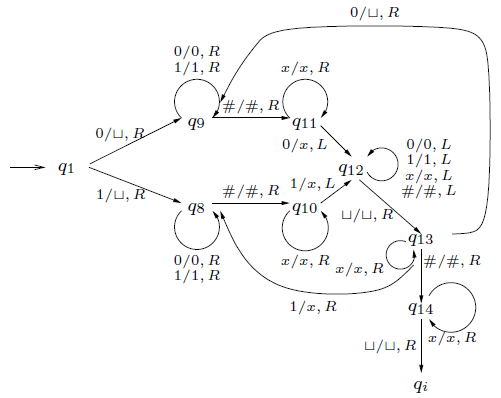
\includegraphics[width=0.6\linewidth]{img/turinggep_pelda}
		\caption{Egy, az $L = \left\{u\#u \ | \ u \in \left\{0,1\right\}^{+}\right\}$ felismerő Turing-gép.}
		\label{fig:turinggep_pelda}
	\end{figure}
	
	\noindent \textbf{Turing-gépek ekvivalenciája}: Két Turing-gépet ekvivalensnek nevezünk, ha ugyanazt a nyelvet ismerik fel.\\

	\noindent \textbf{Turing-felismerhető nyelv, rekurzívan felismerhető nyelvek osztálya}:
	Egy $L \subseteq \Sigma^{*}$ nyelv Turing-felismerhető, ha	$L = L(M)$ valamely $M$ Turing-gépre.
	A Turing-felismerhető nyelveket szokás \textit{rekurzívan felsorolhatónak} is nevezni.
	A rekurzívan felsorolható nyelvek osztályát $RE$-vel jelöljük.\\
	
	\noindent \textbf{Turing-eldönthető nyelv, rekurzív nyelvek osztálya}:
	Egy $L \subseteq \Sigma^{*}$ nyelv Turing-eldönthető, ha létezik olyan Turing-gép,
	amely minden bemeneten megállási konfigurációba jut és felismeri $L$-et.
	A Turing-felismerhető nyelveket szokás \textit{rekurzívnak} is nevezni.
	A rekurzív nyelvek osztályát $R$-rel jelöljük.\\
	
	\noindent \textbf{Turing-gép futási ideje, időigénye}:
	Tekintsünk egy $M = (Q, \Sigma, \Gamma, \delta, q_{0}, q_{i}, q_{n})$ Turing-gépet és annak egy
	$u \in \Sigma^{*}$ bemenő szavát. Azt mondjuk, hogy $M$ futási ideje (időigénye) az $u$ szón $n$ ($n \geq 0$),
	ha $M$ a $q_{0}u\sqcup$ kezdőkonfigurációból $n$ lépésben el tud jutni egy megállási konfigurációba. Ha nincs ilyen
	szám, akkor $M$ futási ideje az $u$ szón végtelen.
	
	Legyen $f : \mathbb{N} \to \mathbb{N}$ egy függvény. Azt mondjuk, hogy $M$ időigénye $f(n)$ (vagy azt, hogy $M$
	egy $f(n)$ időkorlátos gép), ha minden $u \in \Sigma^{*}$ input szóra $M$ időigénye az $u$ szón legfeljebb $f(l(u))$.
	
	\subsubsection{Többszalagos Turing-gépek}
	
	A többszalagos Turing-gépek, értelemszerűen, egynél több szalaggal rendelkeznek.
	Mindegyik szalaghoz tartozik egy-egy író-olvasó fej, melyek egymástól
	függetlenül képesek mozogni a szalagon.\\
	
	\noindent \textbf{Többszalagos Turing-gép definíciója}: Legyen $k > 1$. Egy $k$-szalagos Turing-gép egy olyan
	$M = (Q, \Sigma, \Gamma, \delta, q_{0}, q_{i}, q_{n})$ rendszer, ahol a komponensek a $\delta$ kivételével
	megegyeznek az egyszalagos Turing-gép komponenseivel, $\delta$ pedig a következőképpen adódik.
	$\delta : (Q - \left\{q_{i},q_{n}\right\}) \times \Gamma^{k} \to Q \times \Gamma^{k} \times \left\{L, R, S\right\}^{k}$.
	Legyenek $q, p \in Q$, $a_{1}, a_{2}, ... , a_{k}, b_{1}, b_{2}, ..., b_{k} \in \Gamma$ és
	$D_{1}, D_{2}, ..., D_{k} \in \left\{L, R, S\right\}$. Ha $\delta(q,a_{1}, a_{2}, ... , a_{k}) = (p,b_{1}, b_{2}, ..., b_{k}, D_{1}, D_{2}, ..., D_{k})$, akkor a gép akkor a gép a $q$ állapotból, ha a szalagjain rendre az
	$a_{1}, a_{2}, ... , a_{k}$ betűket olvassa, át tud menni a $p$ állapotba, miközben az
	$a_{1}, a_{2}, ... , a_{k}$ betűket átírja a $b_{1}, b_{2}, ... , b_{k}$ betűkre és a szalagokon a fejeket
	$D_{1}, D_{2}, ... , D_{k}$ irányokba mozgatja.
	
	A többszalagos Turing-gép konfigurációja, a konfigurációátmenet valamint a
	felismert illetve eldöntött nyelv definíciója az egyszalagos eset értelemszerű általánosítása.
	A többszalagos Turing-gép időigényét is az egyszalagoshoz hasonlóan	definiáljuk.\\
	
	\noindent \textbf{Többszalagos és egyszalagos gépek ekvivalenciája}: Minden $k$-szalagos, $f(n)$ időkorlátos Turing-géphez
	van vele ekvivalens $\mathcal{O}(n*f(n))$ időkorlátos egyszalagos Turing-gép.
	
	\subsubsection{Nemdeterminisztikus Turing-gépek}
	
	Egy $M$ nemdeterminisztikus Turing-gép állapotfüggvénye
	$\delta : (Q - \left\{q_{i},q_{n}\right\}) \times \mathcal{P}(\Gamma \to Q \times \Gamma \times \left\{L, R\right\})$
	alakú. Tehát $M$ minden konfigurációjából néhány (esetleg nulla) különböző konfigurációba mehet át.
	Ily módon $M$ számítási sorozatai egy $u$ szón egy fával reprezentálhatók. A fa csúcsa $M$ kezdőkonfigurációja,
	a szögpontjai pedig	$M$ konfigurációi. A fa minden levele megfelel $M$ egy számítási sorozatának az
	$u$-n. $M$ akkor fogadja el $u$-t, ha a fa valamelyik levele elfogadó konfiguráció.
	Nevezzük ezt a most leírt fát az $M$ nemdeterminisztikus számítási fájának az
	$u$-n. Az $M$ által felismert nyelv a determinisztikus esethez hasonlóan definiálható,
	a gép által eldöntött nyelv pedig a következőképpen.\\
	
	\noindent \textbf{Nemdeterminisztikus Turing-gép által eldöntött nyelv}: Azt mondjuk, hogy egy nemdeterminisztikus
	$M$ Turing-gép eldönt egy $L \subseteq \Gamma^{*}$ nyelvet, ha felismeri, és minden $u \in \Sigma{*}$ szóra
	$M$ számítási sorozatai végesek és elfogadási vagy elutasítási konfigurációba vezetnek.\\
	
	\noindent \textbf{Nemdeterminisztikus Turing-gép időigénye}: Legyen $f : \mathbb{N} \to \mathbb{N}$ függvény, $M$
	egy nemdeterminisztikus Turing-gép. Az $M$ időigénye $f(n)$, ha egy $n$ hosszú $u$ bemeneten nincsenek $M$-nek
	$f(n)$-nél hosszabb számítási sorozatai, azaz az $M$ számítási fája az $u$-n legfeljebb $f(n)$ magas.\\
	
	\noindent \textbf{Determinisztikus és nemdeterminisztikus Turing-gépek ekvivalenciája}:
	Minden $M$ nemdeterminisztikus Turing-géphez megadható egy ekvivalens $M'$ determinisztikus Turing-gép.
	Továbbá, ha $M$ $f(n)$ időigényű valamely $f : \mathbb{N} \to \mathbb{N}$ függvényre, akkor
	$M'$ $2^{\mathcal{O}(f(n))}$ időigényű.
	
	\subsection{Eldönthetetlen problémák}
	
	Ebben a fejezetben megmutatjuk, hogy bár a Turing-gép a lehető legáltalánosabb
	algoritmus modell, mégis vannak olyan problémák, melyek nem számíthatók ki Turing-géppel.\\
	
	\noindent \textbf{Emlékeztető}: A rekurzívan felsorolható (Turing-felismerhető) nyelvek osztályát $RE$-vel,
	a rekurzív (Turing-eldönthető) nyelvek osztályát $R$-rel jelöljük.\\
	
	Világos, hogy $R \subseteq RE $. A célunk az, hogy megmutassuk: az $R$ valódi részhalmaza az $RE$-nek,
	azaz van olyan nyelv (probléma) ami	Turing-felismerhető, de nem eldönthető.
	
	Csak olyan Turing-gépeket fogunk vizsgálni, melyek bemenő ábécéje a $\left\{0, 1\right\}$ halmaz.
	Ez nem jelenti az általánosság megszorítását, hiszen ha	találunk egy olyan $\left\{0, 1\right\}$ feletti nyelvet,
	melyet nem lehet eldönteni ilyen Turing-géppel, akkor ezt a nyelvet egyáltalán nem lehet eldönteni.\\
	
	\subsubsection{Turing-gépek kódolása}
	
	A $\left\{0, 1\right\}$ feletti szavak felsorolhatóak (vagyis megszámlálhatóak). Valóban, tekintsük azt a felsorolást,
	amelyben a szavak a	hosszuk szerint követik egymást, és két egyforma hosszú szó közül pedig az van
	előbb, amelyik az alfabetikus rendezés szerint megelőzi a másikat. Ily módon
	a $\left\{0, 1\right\}^{*}$ halmaz elemeinek egy felsorolása a következőképpen alakul: $w_{1} = \varepsilon$,
	$w_{2} = 0$, $w_{3} = 1$, $w_{4} = 00$, $w_{5} = 01$ és így tovább. Ebben a fejezetben tehát a
	$w_{i}$ szóval a $\left\{0, 1\right\}^{*}$ $i$. elemét jelöljük.
	
	Legyen továbbá $M$ egy $\left\{0, 1\right\}$ inputábécé feletti Turing-gép. Van olyan $k > 0$ szám, hogy
	$Q$-t felírhatjuk $Q = \left\{p_{1}, ... p_{k}\right\}$ alakban, ahol $p_{1} = q_{0}$, $p_{k-1} = q_{i}$, $p_{k} = q_{n}$.
	Továbbá, van olyan $m > 0$ szám, hogy $\Gamma$-t felírhatjuk $\Gamma = \left\{X_{1}, ... X_{m}\right\}$ alakban,
	ahol $X_{1} = 0$, $X_{2} = 1$, $X_{3} = \sqcup$, és $X_{4}, ... X_{m}$ az $M$ további szalagszimbólumai.
	Nevezzük végül az $L, R, S$ szimbólumokat (amelyek irányokat jelölnek) rendre $D_{1}$, $D_{2}$ és $D_{3}$-nak.
	Ezek után $M$ egy $\delta(p_{i},X_{j}) = (p_{r}, X_{s}, D_{t})$ ($0 \leq i,r \leq k$, $1 \leq j,s \leq m$ és $1 \leq t \leq 3$)
	átmenete elkódolható a $0^{i}10^{j}10^{r}10^{s}10^{t}$ szóval. Mivel minden $0$-s blokk hossza legalább $1$, az átmenetet
	kódoló szóban nem szerepel az $11$ részszó. Tehát az M összes átmenetét kódoló szavakat összefűzhetjük egy olyan szóvá,
	melyben az átmeneteket az $11$ részszó választja el egymástól. Az így kapott szó pedig magát $M$-et kódolja.\\
	
	A továbbiakban $M_{i}$-vel jelöljük azt a Turing-gépet, amelyet a $w_{i}$ szó kódol ($i \geq 1$). Amennyiben
	$w_{i}$ nem a fent leírt kódolása egy Turing-gépnek, akkor tekintsük $M_{i}$-t olyannak, ami minden input esetén
	azonnal a $q_{n}$ állapotba megy, azaz $L(M_{i}) = \emptyset$.\\
	
	A későbbiekben szükségünk lesz arra, hogy elkódoljunk egy $(M, w)$ Turing-gép és bemenet
	párost egy $\left\{0, 1\right\}$ feletti szóban. Mivel a Turing-gépek kódolása nem tartalmazhat
	$111$-et, ezért $(M, w)$ kódja a következő: $M$ kódja után írunk $111$-et, majd utána $w$-t.
	
	\subsubsection{Egy nem rekurzívan felsorolható nyelv}
	
	\noindent \textbf{Az $L_{\acute{a}tl\acute{o}}$ nyelv}: Az $L_{\acute{a}tl\acute{o}}$ nyelv azon $\left\{0, 1\right\}$
	feletti Turing-gépek bináris kódjait tartalmazza, melyek nem fogadják el önmaguk kódját, mint bemenő szót, azaz
	$L_{\acute{a}tl\acute{o}} = \left\{w_{i} \ | \ i \geq 1, w_{i} \notin L(M_{i}) \right\}$\\
	
	\noindent \textbf{Tétel}: $L_{\acute{a}tl\acute{o}} \notin RE$.
	
	\subsubsection{Egy rekurzívan felsorolható, de nem eldönthető nyelv}
	
	\noindent \textbf{Az $L_{u}$ nyelv}: Tekintsük azon $(M, w)$ párok halmazát (egy megfelelő bináris szóban elkódolva),
	ahol $M$ egy $\left\{0, 1\right\}$	bemenő ábécé feletti Turing-gép, $w$ pedig egy $\left\{0, 1\right\}$ feletti
	szó úgy, hogy $w \in L(M)$, azaz $M$ elfogadja $w$-t. Ezt a nyelvet jelöljük $L_{u}$-val.
	$L_{u} = \left\{\langle w_{i},w_{j} \rangle \ | \ i, j \geq 1, w_{j} \in L(M_{i}) \right\}$\\
	
	\noindent \textbf{Tétel}: $L_{u} \in RE$.\\
	
	\noindent \textbf{Tétel}: $L_{u} \notin R$.
	
	\subsubsection{További tételek}
	
	\begin{enumerate}
		\item	Legyen $L$ egy nyelv. Ha $L, \bar{L} \in RE$, akkor $L \in R$. Következmény: a rekurzívan felsorolható
		nyelvek nem zártak a komplementerképzésre.
		
		\item	Ha $L \in R$, akkor $\bar{L} \in R$, azaz a rekurzív nyelvek zártak a komplementerképzésre.
	\end{enumerate}
	
	\subsubsection{További eldönthetetlen problémák}
	
	\noindent \textbf{Kiszámítható függvény}: Legyen $\Sigma$ és $\Delta$ két ábécé és $f$ $\Sigma^{*}$ból
	$\Delta^{*}$-ba képző függvény. Azt mondjuk, hogy $f$ kiszámítható, ha van olyan $M$ Turing-gép, hogy
	$M$-et egy $w \in \Sigma^{*}$ szóval a bemenetén elindítva, $M$ úgy áll meg, hogy a szalagján a
	$f(w) \in \Delta^{*}$ szó van.\\
	
	\noindent \textbf{Eldöntési problémák visszavezetése}: Legyen $L_{1} \subseteq \Sigma^{*}$ és $L_{2} \subseteq \Delta^{*}$
	két eldöntési probléma. $L_{1}$ visszavezethető $L_{2}$-re ($L_{1} \leq L_{2}$), ha van olyan
	$f : \Sigma^{*} \to \Delta^{*}$ kiszámítható függvény, hogy minden $w \in \Sigma^{*}$ szóra
	$w \in L_{1}$ pontosan akkor teljesül, ha $f(w) \in L_{2}$ is teljesül.\\
	
	\noindent \textbf{Tétel}: Legyen $L_{1} \subseteq \Sigma^{*}$ és $L_{2} \subseteq \Delta^{*}$
	két eldöntési probléma és tegyük fel, hogy $L_{1}$ visszavezethető $L_{2}$-re. Ekkor igazak a következő állítások:
	
	\begin{enumerate}
		\item	Ha $L_{1}$ eldönthetetlen, akkor $L_{2}$ is.
		
		\item	Ha $L_{1} \notin RE$ , akkor $L_{2} \notin RE$.
	\end{enumerate}
	
	\noindent \textbf{A megállási probléma}: Legyen $L_{h} = \left\{\langle M, w \rangle \ |\ M \ meg\acute{a}ll \ a \ w \ bemeneten \right\}$,
	azaz $L_{h}$ azon $\langle M, w \rangle$ Turing-gép és bemenet párosokat tartalmazza elkódolva, melyekre $M$ megáll a $w$ bemeneten.
	$L_{h}$ eldönthetetlen ($L_{u}$ visszavezethető $L_{h}$-ra), viszont $L_{h} \in RE$.\\
	
	\noindent \textbf{Az $L_{\ddot{u}res}$ probléma}: Legyen $L_{\ddot{u}res} = \left\{\langle M \rangle \ |\ L(M) = \emptyset \right\}$.
	$L_{\ddot{u}res}$ eldönthetetlen ($L_{u}$ visszavezethető $L_{\ddot{u}res}$-re), valamint $L_{\ddot{u}res} \notin RE$.\\
	
	\noindent \textbf{Rekurzívan felsorolható nyelvek (nem triviális) tulajdonsága}: Ha $\mathcal{P}$ a rekurzívan felsorolható
	nyelvek egy halmaza, akkor $\mathcal{P}$ a rekurzívan felsorolható nyelvek egy tulajdonsága. Ha $\mathcal{P} \not = \emptyset$ és
	$\mathcal{P} \not = RE$, akkor $\mathcal{P}$ nem triviális tulajdonsága a rekurzívan felsorolható nyelveknek.\\
	
	\noindent \textbf{Rice tétele}: 
	Adott $\mathcal{P}$ tulajdonságra jelöljük $L_{\mathcal{P}}$-vel azon Turing-gépek kódjainak halmazát, amelyek
	$\mathcal{P}$-beli nyelvet ismernek fel. Ha $\mathcal{P}$ a rekurzívan felsorolható nyelvek egy nem triviális tulajdonsága, akkor
	$L_{\mathcal{P}}$ eldönthetetlen.\\
	
	\noindent \textbf{Post Megfelelkezési Probléma (röviden PMP)}: A PMP problémát a következőképpen definiáljuk. Legyen
	$\Sigma$ egy legalább két betűt tartalmazó ábécé és legyen $D = \left\{[\frac{u_{1}}{v_{1}}], ..., [\frac{u_{n}}{v_{n}}]\right\}$
	egy dominóhalmaz, melyben $n \geq 1$ és $u_{1}, ..., u_{n}, v_{1}, ..., v_{n} \in \Sigma^{+}$. A kérdés az,	hogy van-e egy olyan
	$1 \leq i_{1}, ..., i_{m} \leq m$ ($m \geq 1$) indexsorozat, melyre teljesül, hogy a $[\frac{u_{i_{1}}}{v_{i_{1}}}], ..., [\frac{u_{i_{m}}}{v_{i_{m}}}]$ dominókat egymás mellé írva alul és felül ugyanaz a szó adódik, azaz
	$u_{i_{1}} ... u_{i_{m}} = v_{i_{1}} ... v_{i_{m}}$. Ebben az esetben a fenti dominósorozatot a D egy megoldásának nevezzük.
	
	Formális nyelvként a következőképpen definiálhatjuk a PMP-t:
	PMP $= \left\{ \langle D \rangle \ |\ D-nek \ van \ megold\acute{a}sa \right\}$. PMP eldönthetetlen.
		
	\subsection{Bonyolultságelmélet}
	
	A bonyolultságelmélet célja a megoldható (és ezen belül az eldönthető) problémák osztályozása a megoldáshoz szükséges
	erőforrások (jellemzően az idő és a tár) mennyisége szerint.
	
	\subsubsection{Időbonyolultsági fogalmak}
	
	\noindent \textbf{TIME}: Legyen $f : \mathbb{N} \to \mathbb{N}$ függvény. \textbf{TIME}($f(n)$) $= \left\{L \ | \ L \ eld\ddot{o}nthet\tilde{o} \ \mathcal{O}(f(n)) \ id\tilde{o}ig\acute{e}ny\tilde{u} \ Turing-g\acute{e}ppel \right\}$\\
	
	\noindent \textbf{P} $=\bigcup_{k \geq 1}$ \textbf{TIME}($n^{k}$). Tehát \textbf{P} azon nyelveket tartalmazza,
	melyek eldönthetőek polinom időkorlátos	determinisztikus Turing-géppel. Ilyen például a jól ismert \textsc{Elérhetőség}
	probléma, melynek bemenete egy $G$ gráf és annak két kitüntetett csúcsa ($s$ és $t$). A	kérdés az, hogy van-e a $G$-ben
	út $s$-ből $t$-be. Ha az \textsc{Elérhetőség} problémára nyelvként tekintünk, akkor írhatjuk azt, hogy\\
	
	\textsc{Elérhetőség} $= \left\{\langle G, s, t \rangle \ | \ G-ben \ van \ \acute{u}t \ s-b\tilde{o}l \ t-be\right\}$.\\
	
	Könnyen megadható az \textsc{Elérhetőség} problémáját polinom időben eldöntő determinisztikus Turing-gép, tehát
	\textsc{Elérhetőség} $\in$ \textbf{P}.\\
	
	\noindent \textbf{NTIME}: Legyen $f : \mathbb{N} \to \mathbb{N}$ függvény.\\ \textbf{NTIME}($f(n)$) $= \left\{L \ | \ L \ eld\ddot{o}nthet\tilde{o} \ \mathcal{O}(f(n)) \ id\tilde{o}ig\acute{e}ny\tilde{u} \ nemdeterminisztikus\ Turing-g\acute{e}ppel \right\}$\\
		
	\noindent \textbf{NP} $=\bigcup_{k \geq 1}$ \textbf{NTIME}($n^{k}$).
	Az \textbf{NP}-beli problémák rendelkeznek egy közös tulajdonsággal az alábbi értelemben.
	Ha tekintjük egy \textbf{NP}-beli probléma egy példányát és egy lehetséges "bizonyítékot"
	arra nézve, hogy ez a példány "igen" példánya az adott problémának,
	akkor ezen bizonyíték helyességének leellenőrzése polinom időben elvégezhető.
	Ennek megfelelően egy \textbf{NP}-beli problémát eldöntő nemdeterminisztikus Turing-gép
	általában úgy működik, hogy "megsejti" a probléma bemenetének egy lehetséges megoldását,
	és polinom időben leellenőrzi, hogy a megoldás helyes-e.
	
	Tekintsük a \textsc{Sat} problémát, amit a következőképpen definiálunk. Adott egy $\phi$ ítéletlogikai KNF.
	A kérdés az, hogy kielégíthető-e. Annak a bizonyítéka, hogy	a $\phi$ kielégíthető, egy olyan változó-hozzárendelés,
	ami mellett kiértékelve a $\phi$-t igaz értéket kapunk. Egy tetszőleges változó-hozzárendelés tehát a $\phi$
	kielégíthetőségének egy lehetséges bizonyítéka .Annak leellenőrzése pedig, hogy ez a
	hozzárendelés tényleg igazzá teszi-e $\phi$-t, polinom időben elvégezhető. A \textsc{Sat}
	\textbf{NP}-beli probléma.\\
	
	\noindent Az a definíciókból következik, hogy fennáll a \textbf{P} $\subseteq$ \textbf{NP} tartalmazás.
	
	\subsubsection{NP-teljes problémák}
	
	\noindent \textbf{Polinom időben kiszámítható függvény}: Legyen $\Sigma$ és $\Delta$ két ábécé és $f$ $\Sigma^{*}$ból
	$\Delta^{*}$-ba képző függvény. Azt mondjuk, hogy $f$ polinom időben kiszámítható, ha kiszámítható egy polinom
	időigényű Turing-géppel.\\
	
	\noindent \textbf{Eldöntési problémák polinom idejű visszavezetése}:
	Legyen $L_{1} \subseteq \Sigma^{*}$ és $L_{2} \subseteq \Delta^{*}$	két eldöntési probléma.
	$L_{1}$ polinom időben visszavezethető $L_{2}$-re ($L_{1} \leq_{p} L_{2}$), ha $L_{1} \leq L_{2}$ és
	a visszavezetésben használt $f$ függvény polinom időben kiszámítható.\\
	
	\noindent \textbf{Tétel}: Legyen $L_{1}$ és $L_{2}$ két probléma úgy, hogy $L_{1} \leq_{p} L_{2}$. Ha $L_{2}$
	
	\begin{enumerate}
		\item	\textbf{P}-beli, akkor $L_{1}$ is \textbf{P}-beli.
		
		\item	\textbf{NP}-beli, akkor $L_{1}$ is \textbf{NP}-beli.
	\end{enumerate}
	
	\noindent \textbf{NP-teljes probléma}: Legyen $L$ egy probléma. Azt mondjuk, hogy $L$ \textbf{NP}-teljes, ha
	
	\begin{enumerate}
		\item	\textbf{NP}-beli, és
		
		\item	minden további \textbf{NP}-beli probléma polinom időben visszavezethető $L$-re.
			
	\end{enumerate}
	
	\noindent \textbf{Tétel}: Legyen $L$ egy \textbf{NP}-teljes probléma. Ha $L \in$ \textbf{P}, akkor \textbf{P} $=$ \textbf{NP}.\\
	
	\noindent \textbf{Megjegyzés}: Jelenleg \textbf{NEM} tudunk \textbf{P}-beli \textbf{NP}-teljes problémáról!!!\\
	
	\noindent \textbf{Tétel}: Legyen $L_{1}$ egy \textbf{NP}-teljes, $L_{2}$ pedig \textbf{NP}-beli probléma.
	Ha $L_{1} \leq_{p} L_{2}$, akkor $L_{2}$ is \textbf{NP}-teljes.\\
	
	\noindent \textbf{Cooke tétele}: \textsc{Sat} \textbf{NP}-teljes.\\
	
	\noindent Legyen $k \geq 1$.
	k\textsc{Sat} $= \left\{\langle \phi \rangle \ | \ \phi \ minden \ tagj\acute{a}ban \ k \ liter\acute{a}l \ van. \right\}$\\
	
	\noindent \textbf{Tétel}: 3\textsc{Sat} \textbf{NP}-teljes, ugyanis \textsc{Sat} $\leq_{p}$ 3\textsc{Sat}.\\
	
	\noindent \textsc{Teljes részgráf} $= \left\{\langle G, k \rangle \ | \ G \ v\acute{e}ges \ gr\acute{a}f, k \geq 1, \ G-nek \ \exists \ k
	\ cs\acute{u}cs\acute{u} \ r\acute{e}szgr\acute{a}fja  \right\}$.
	Tehát a \textsc{Teljes részgráf} azon $G$ és $k$ párokat tartalmazza, megfelelő ábécé feletti
	szavakban elkódolva, melyekre igaz, hogy $G$-ben van $k$ csúcsú teljes részgráf,
	azaz olyan részgráf, melyben bármely két csúcs között van él.\\

	\noindent \textsc{Teljes részgráf}$= \left\{\langle G, k \rangle \ | \ G \ v\acute{e}ges \ gr\acute{a}f, k \geq 1, \ G-nek \ \exists \ k
	\ cs\acute{u}cs\acute{u} \ r\acute{e}szgr\acute{a}fja  \right\}$.
	Tehát a \textsc{Teljes részgráf} azon $G$ és $k$ párokat tartalmazza, megfelelő ábécé feletti
	szavakban elkódolva, melyekre igaz, hogy $G$-ben van $k$ csúcsú teljes részgráf,
	azaz olyan részgráf, melyben bármely két csúcs között van él.\\
	
	\noindent \textsc{Független csúcshalmaz} $= \left\{\langle G, k \rangle \ | \ G \ v\acute{e}ges \ gr\acute{a}f, k \geq 1, \ G-nek \ \exists \ k	\ elem\tilde{u} \ f\ddot{u}ggetlen \ cs\acute{u}cshalmaza  \right\}$.
	Vagyis a  \textsc{Független csúcshalmaz} azon $G$ és $k$ párokat tartalmazza, melyekre
	igaz, hogy $G$-ben van $k$ olyan csúcs, melyek közül egyik sincs összekötve a
	másikkal.\\
	
	\noindent \textsc{Csúcslefedés} $=$\\
	$\left\{\langle G, k \rangle \ | \begin{array}{lr}
	\ G \ v\acute{e}ges \ gr\acute{a}f, k \geq 1, \ G-nek \ van \ olyan \ k	\ elem\tilde{u} \ cs\acute{u}cshalmaza,\\
	mely \ tartalmazza \ G \ minden \ \acute{e}l\acute{e}nek \ legal\acute{a}bb \ 1 \ v\acute{e}gpontj\acute{a}t.
	\end{array}
	\right\}$.\\
	
	
	\noindent \textsc{Teljes részgráf}, \textsc{Független csúcshalmaz} és \textsc{Csúcslefedés} \textbf{NP}-teljesek
	(\textsc{Teljes részgráf} $\leq_{p}$ \textsc{Független csúcshalmaz} $\leq_{p}$ \textsc{Csúcslefedés}).\\
	
	\noindent \textsc{Utazóügynök} $=$\\
	$\left\{\langle G, k \rangle \ |
	\begin{array}{lr}
	 \ G \ v\acute{e}ges \ ir\acute{a}ny\acute{i}tatlan \ gr\acute{a}f, \ az \ \acute{e}leken \ egy-egy \
	pozit\acute{i}v \ eg\acute{e}sz \ s\acute{u}llyal \ \acute{e}s \\
	van \ G-ben \ legfeljebb \ k \ \ddot{o}sszs\acute{u}ly\acute{u} \ Hamilton \ k\ddot{o}r
	\end{array}
	 \right\}$.\\	
	 
	\noindent \textbf{Tétel}: Az \textsc{Utazóügynök} probléma \textbf{NP}-teljes.
	
	\subsubsection{Tárbonyolultság}
	A tárbonyolultságot egy speciális, úgynevezett offline Turing-gépen vizsgáljuk.\\
	
	\noindent \textbf{Off-line Turing-gép}: Offline Turing-gépnek nevezünk egy olyan többszalagos Turing-gépet,
	mely a bemenetet tartalmazó szalagot csak olvashatja, a többi, ún. munkaszalagokra
	pedig írhat is. Az offline Turing-gép tárigényébe csak a munkaszalagokon
	felhasznált terület számít be.\\
	
	A továbbiakban Turing-gép alatt minidig offline Turing-gépet értünk. Most
	definiáljuk a tárbonyolultsággal kapcsolatos nyelvosztályokat.\\
	
	\noindent \textbf{SPACE}(f(n)) = $\left\{L|L \ eld\ddot{o}nthet\tilde{o} \ \mathcal{O}(f(n)) \ t\acute{a}rig\acute{e}ny\tilde{u} \
	determinisztikus \ Turing-g\acute{e}ppel \right\}$\\
	
	\noindent \textbf{NSPACE}(f(n)) = $\left\{L|L \ eld\ddot{o}nthet\tilde{o} \ \mathcal{O}(f(n)) \ t\acute{a}rig\acute{e}ny\tilde{u} \
	nemdeterminisztikus \ Turing-g\acute{e}ppel \right\}$\\
	
	\noindent \textbf{PSPACE} $=\bigcup_{k > 0}$ \textbf{SPACE}($n^{k}$)\\
	
	\noindent \textbf{NPSPACE} $=\bigcup_{k > 0}$ \textbf{NSPACE}($n^{k}$)\\
	
	\noindent \textbf{L} $=$ \textbf{SPACE}($\log_{2} n$) \\
	
	\noindent \textbf{NL} $=$ \textbf{NSPACE}($\log_{2} n$) \\
	
	\noindent \textbf{Savitch tétele}: Ha $f(n) \geq \log n$, akkor \textbf{NSPACE}($f(n)$) $\subseteq$ \textbf{SPACE}($f^{2}(n)$).
\end{document}